% TODO: stichpunkte als fließtext soweit möglich (reflexion & fazit). vielleicht auch in anderen abschnitten (kapitel 2, ab seite 10).

\subsection{Prompt-Setup: Einheitliche Aufgabenstellung für alle Tools}
\label{sec:prompt-setup}

Um eine objektive und vergleichbare Bewertung zu ermöglichen, wurde für die
Implementierung des Map-Screens in allen drei Tools (\textit{GitHub Copilot},
\textit{Cursor}, \textit{Bolt.new}) derselbe, detaillierte Prompt verwendet,
der die funktionalen und technischen Anforderungen klar definierte:

\begin{lstlisting}[]
    Create a Map Screen with Event Markers and Filter in React Native
    
    Create a React Native component called `MapScreen` that displays event markers on a map using event data from the `EventsProvider` context.
    
    ## Requirements
    
    ### Functionality
    - Use the list of events from the `EventsProvider` context.  
      (Access: `const { events, loading, error, refreshEvents } = useEvents();`)
    - Each event contains:
      - `docId: string`
      - `title: string`
      - `category: string`
      - `date: string`
      - `geoPoint: { latitude: number; longitude: number }`
    - Example Context Usage: const { events, loading, error, refreshEvents } = useEvents();
    - Display all events as markers on a map (`react-native-maps` or Expo MapView).
    - When a marker is tapped, show a callout or modal with event details (`title`, `time`, `category`, optional image/avatar).
    - Add filter options above the map (e.g. by category, date, distance).  
      Only display events that match active filters.
    - Handle loading and error states appropriately.
    
    ### UI/UX
    - Modern mobile UI with a clean filter bar on top, responsive marker popups, and a loading spinner.
    - Use functional components and React hooks (TypeScript).
    - Styling should be clean and minimal (simple css with StyleSheet prefered).
    - Map should fit all visible markers and allow user zoom/pan.
    - Compatible with Expo.
    
    ### File Structure
    - Main screen in `map.tsx`.
    - Optional: Reusable `EventMarker` component.
    
    ### Additional
    - Keep code modular, clean, and well-commented.
    - Focus on maintainability and clarity.
    - Use the attached layout (filter bar on top, map below, details as bottom sheet/callout) as a visual reference.
    
    ### Example Event Type (TypeScript)
    interface Event {
      docId: string;
      title: string;
      category: string;
      date: string;
      geoPoint: { latitude: number; longitude: number };
      // ...more fields possible
    }

    ## Goal
    A fully functional, modern React Native map screen with event markers, filter bar, marker popups, and proper handling of loading/error states -- ready to integrate into an Expo app.

    
    \end{lstlisting}

\noindent
\textbf{Hinweis:} Diese Aufgabenstellung wurde in allen Demonstrationen identisch genutzt, um die Unterschiede in Lösungsstrategie und Codequalität der Tools direkt vergleichbar zu machen.

\subsection{Demonstration mit GitHub Copilot}

\subsubsection{Setup und Vorgehen}
Die Entwicklung des Map-Screens wurde exemplarisch mit \textbf{GitHub Copilot}
in Visual Studio Code durchgeführt. Für größtmögliche Vergleichbarkeit kamen
ausschließlich die Copilot-Funktionen zum Einsatz, keine weiteren KI-Plugins.

\begin{figure}[htbp]
      \centering
      \vspace{1em}
      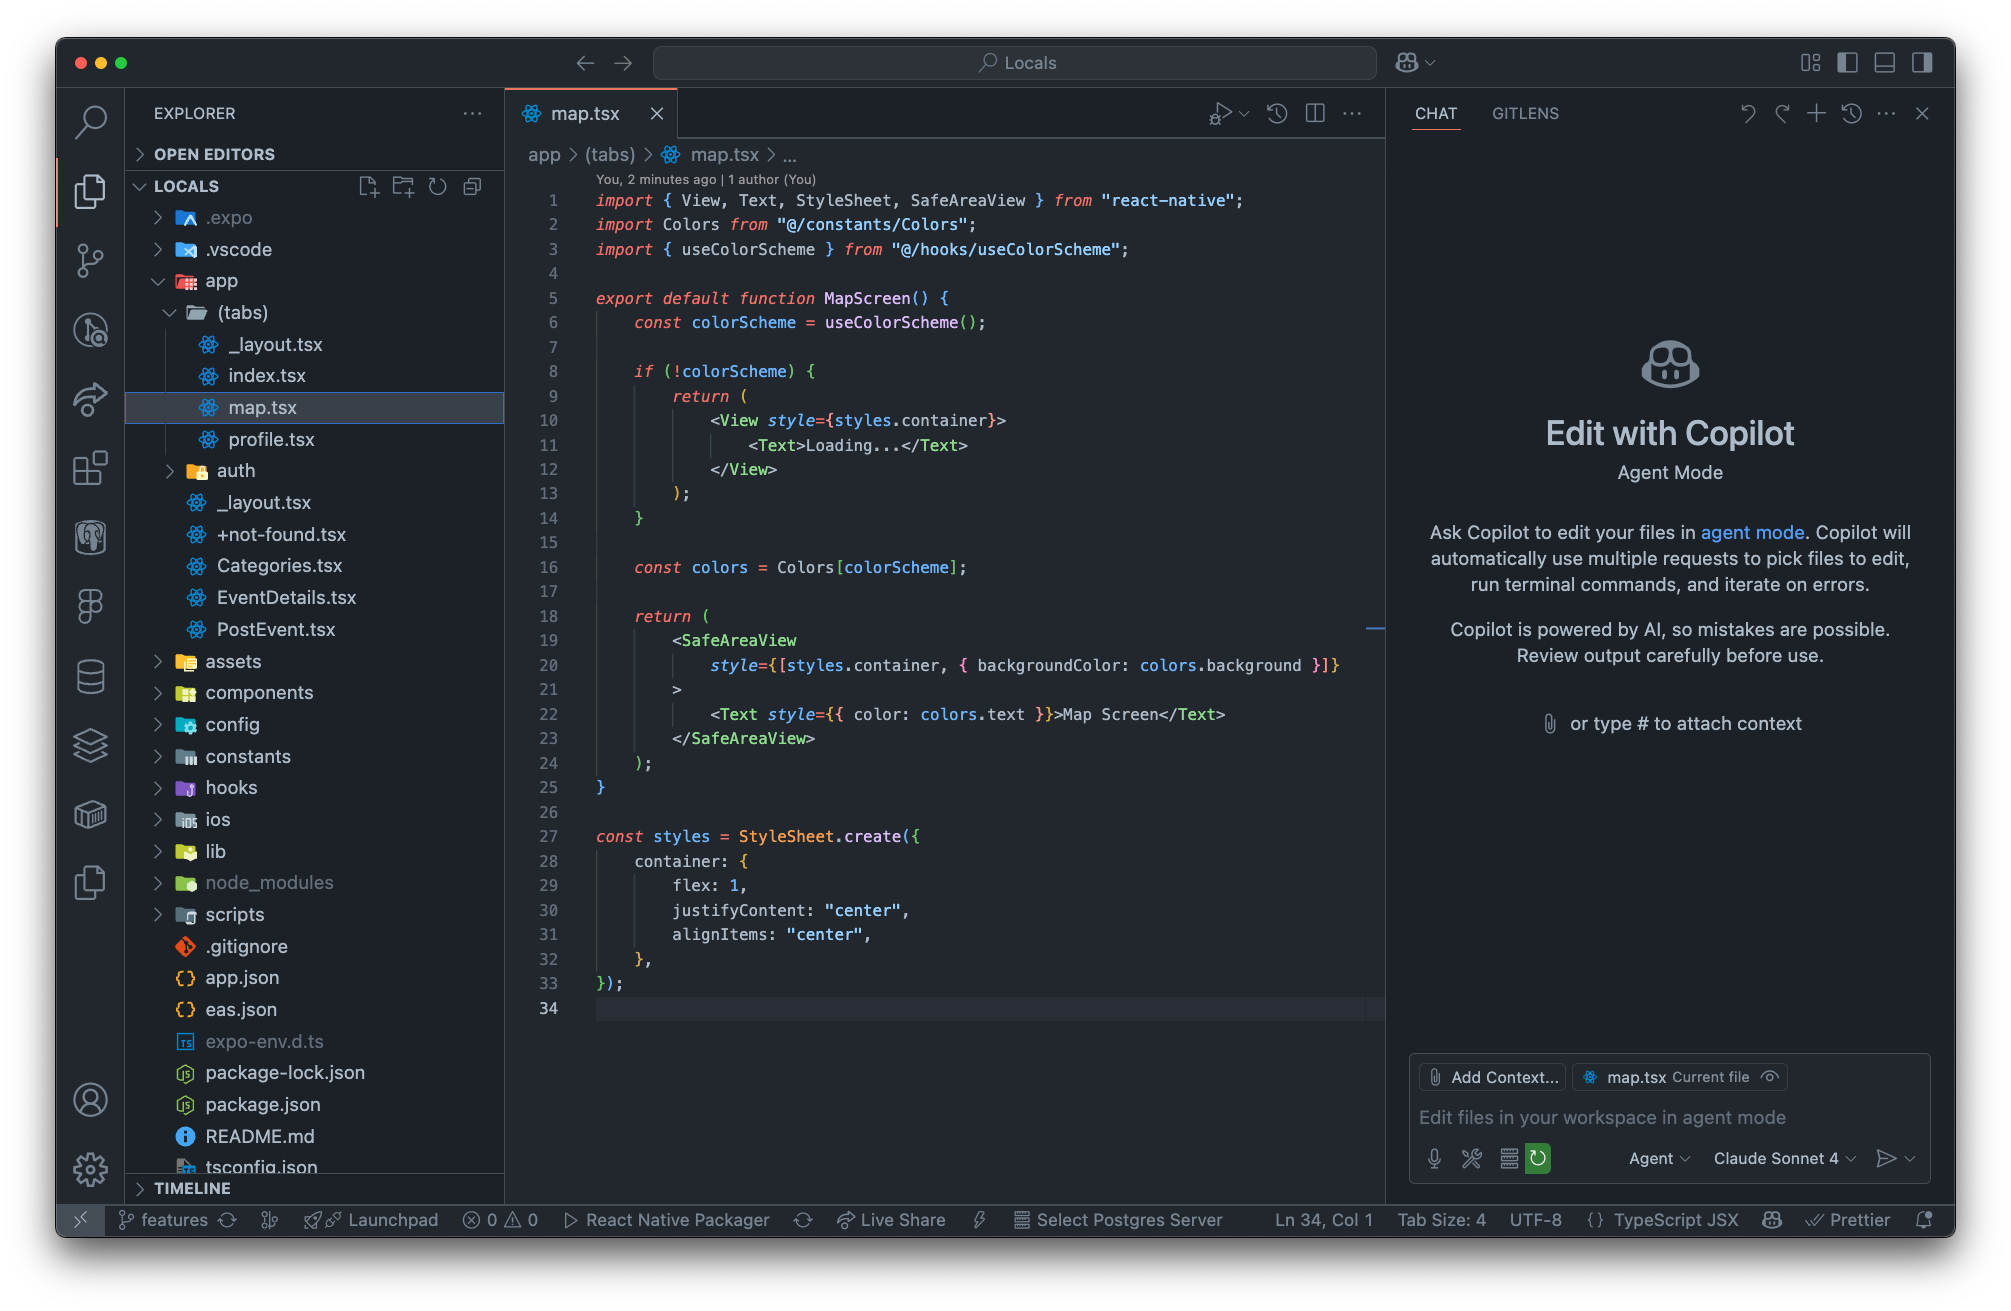
\includegraphics[width=1\textwidth]{images/copilot_screenshots/Screenshots Ist-Zustand-copilot.png}
      \caption{Ausgangszustand der Anwendung vor dem Einsatz von Copilot. \textit{Copilot-Demo}}
      \label{fig:copilot-istzustand}
\end{figure}

% TODO: muss ich alles aufzählen nicht nur z.b.?
Zu Beginn wurde die Entwicklungsumgebung vorbereitet (z.~B.\ Installation von
\texttt{react-native-maps} und \texttt{expo-location}). Die Aufgabenstellung
wurde als Kommentar oder Docstring auf Englisch eingefügt (\emph{siehe
      Abschnitt~\ref{sec:prompt-setup}}).

\subsubsection{Schrittweise Umsetzung und Reflexion}
Die Entwicklung erfolgte nach folgendem Muster:
\begin{enumerate}
      \item \textbf{Prompt definieren:} Pro Feature (z.\,B. Marker, Filter, Event-Details) wurde ein spezifischer Kommentar als Arbeitsanweisung eingefügt.
      \item \textbf{Vorschläge von Copilot akzeptieren oder anpassen:} Vorschläge wurden übernommen, angepasst oder verworfen.
      \item \textbf{Test und Dokumentation:} Nach jeder Änderung wurde der Code getestet und die Funktionsweise reflektiert.
      \item \textbf{Fehlersuche und Nacharbeit:} Fehlerhafte Vorschläge oder Bugs wurden durch Rücksprache mit Copilot, Recherche oder manuelle Nacharbeit behoben.
\end{enumerate}

\begin{figure}[htbp]
      \centering
      \vspace{1em}
      \begin{minipage}{0.48\textwidth}
            \centering
            \includegraphics[width=0.98\textwidth]{images/copilot_screenshots/implementation-rückmeldung-copilot-1.png}
      \end{minipage}
      \hfill
      \begin{minipage}{0.48\textwidth}
            \centering
            \includegraphics[width=0.98\textwidth]{images/copilot_screenshots/implementation-rückmeldung-copilot-2.png}
      \end{minipage}
      \caption{Rückmeldung und Hinweise von Copilot während der Implementierung. \textit{Copilot-Demo}}
      \label{fig:copilot-impl-pair}
\end{figure}

\noindent Die technische Umsetzung umfasste:
\begin{itemize}
      \item Anzeige aller Events als Marker (mit Kategorie und Titel) auf der Karte.
      \item Filterleiste zur Auswahl nach Kategorie und Datum.
      \item Darstellung von Event-Details beim Tippen auf einen Marker.
      \item Responsives Layout, modernes UI-Design, Fehler- und Ladezustände.
\end{itemize}

\begin{figure}[htbp]
      \centering
      \vspace{1em}
      \begin{minipage}{0.48\textwidth}
            \centering
            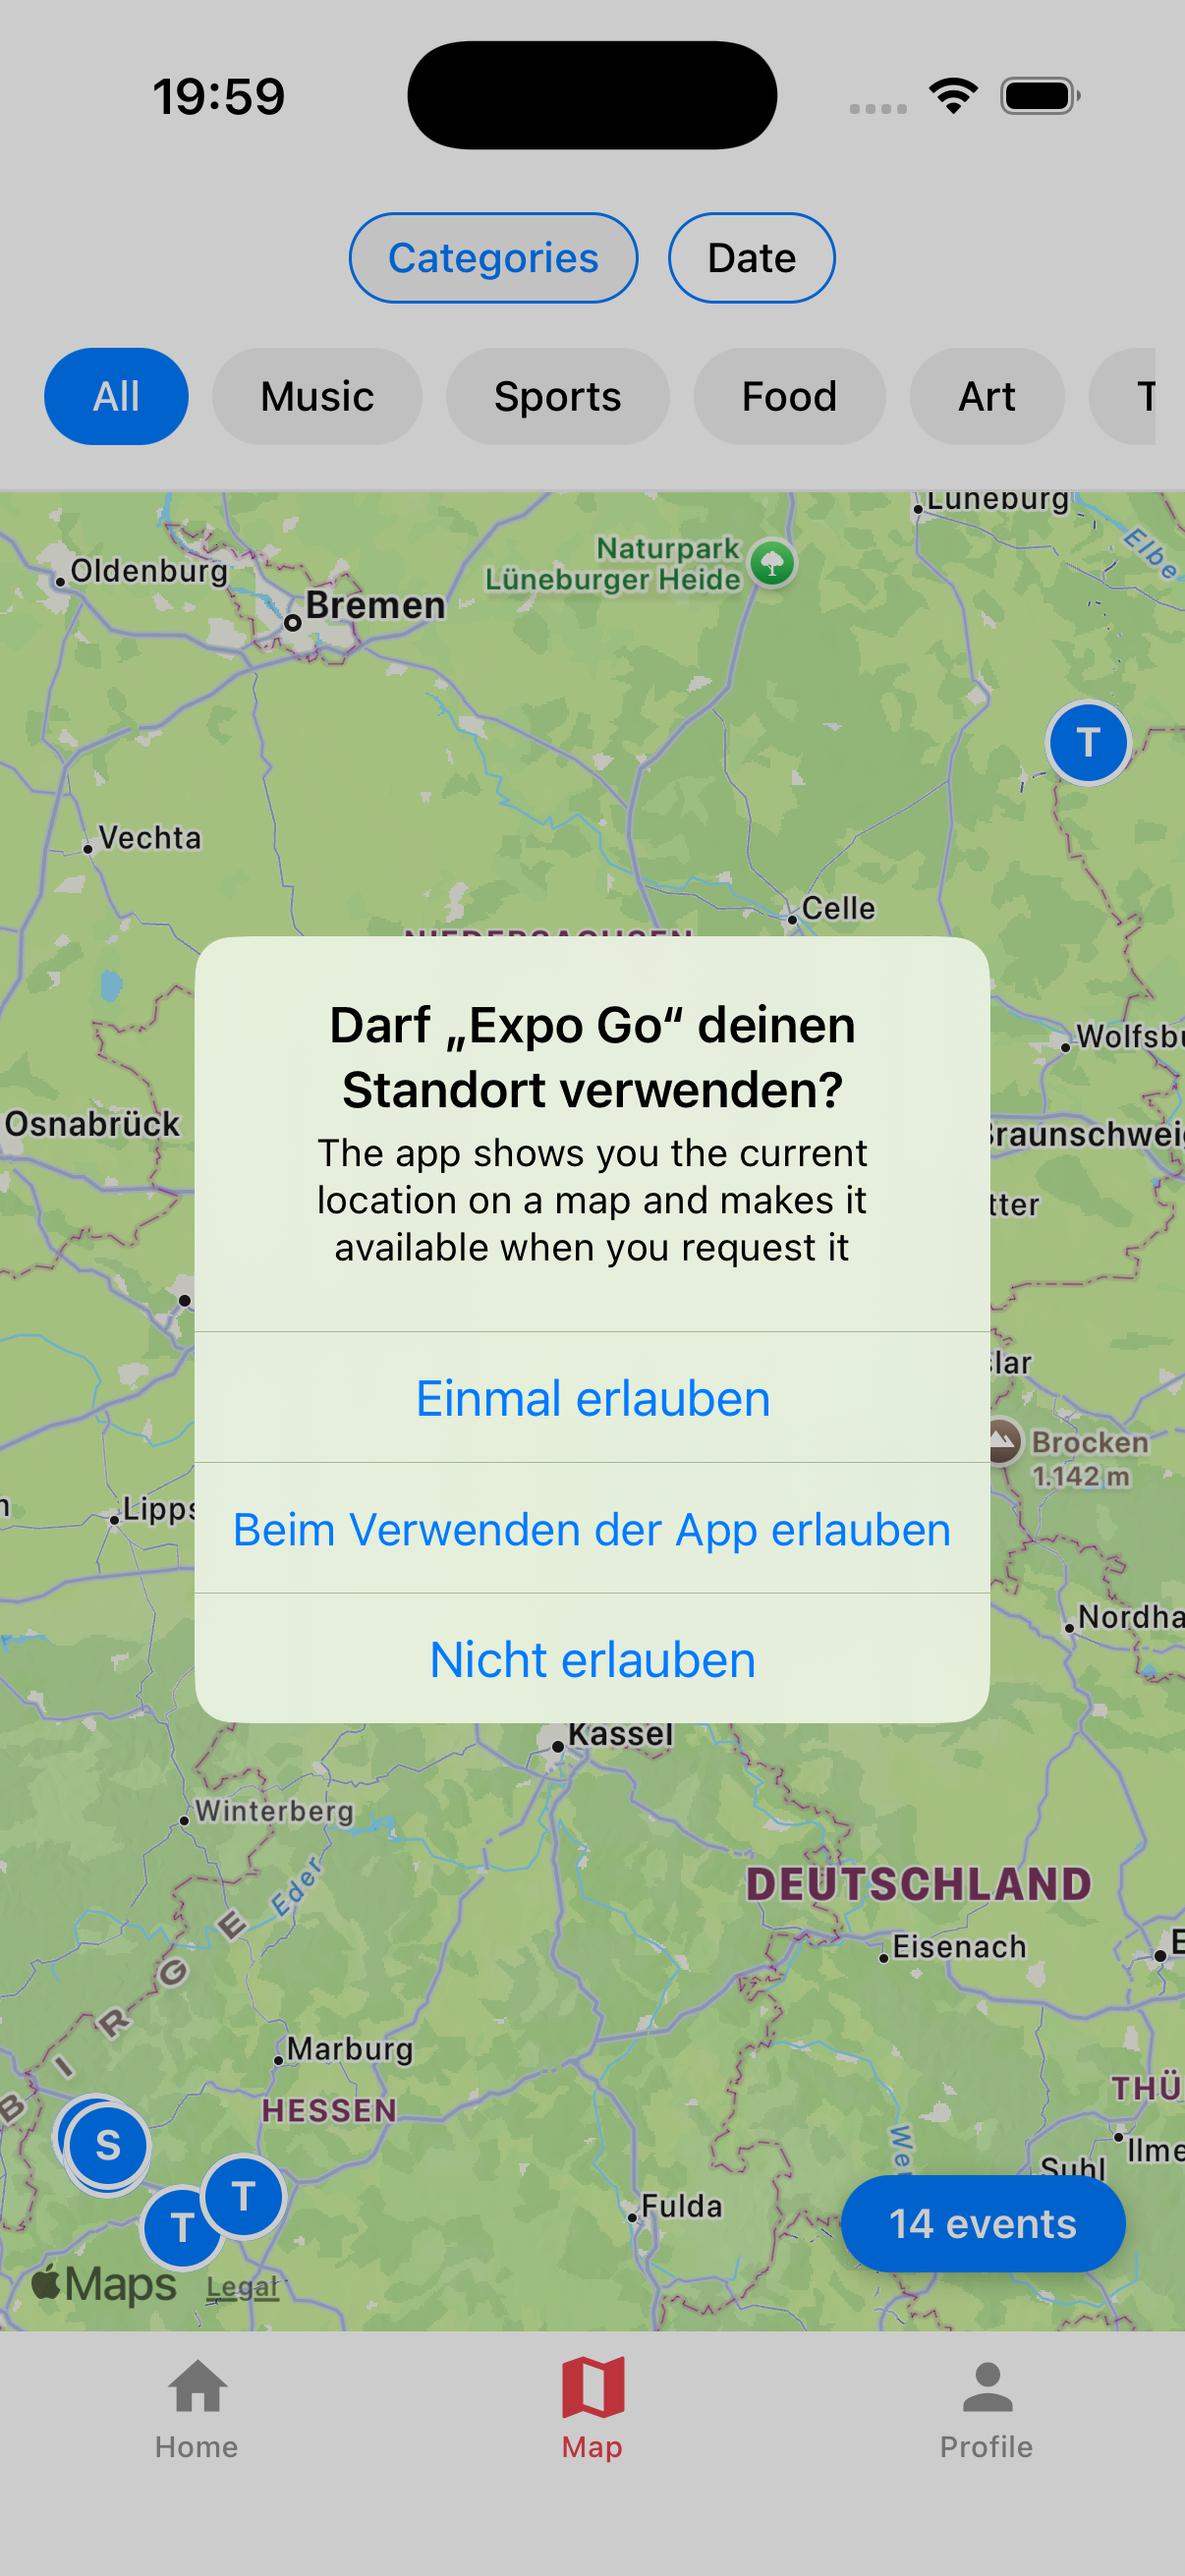
\includegraphics[width=\textwidth]{images/copilot_screenshots/6. 1. Version das MapScreens - Screenshot-copilot.png}
            \caption{Erste lauffähige Version des MapScreens nach KI-gestützter Entwicklung. \textit{Copilot-Demo}}
      \end{minipage}
      \hfill
      \begin{minipage}{0.48\textwidth}
            \centering
            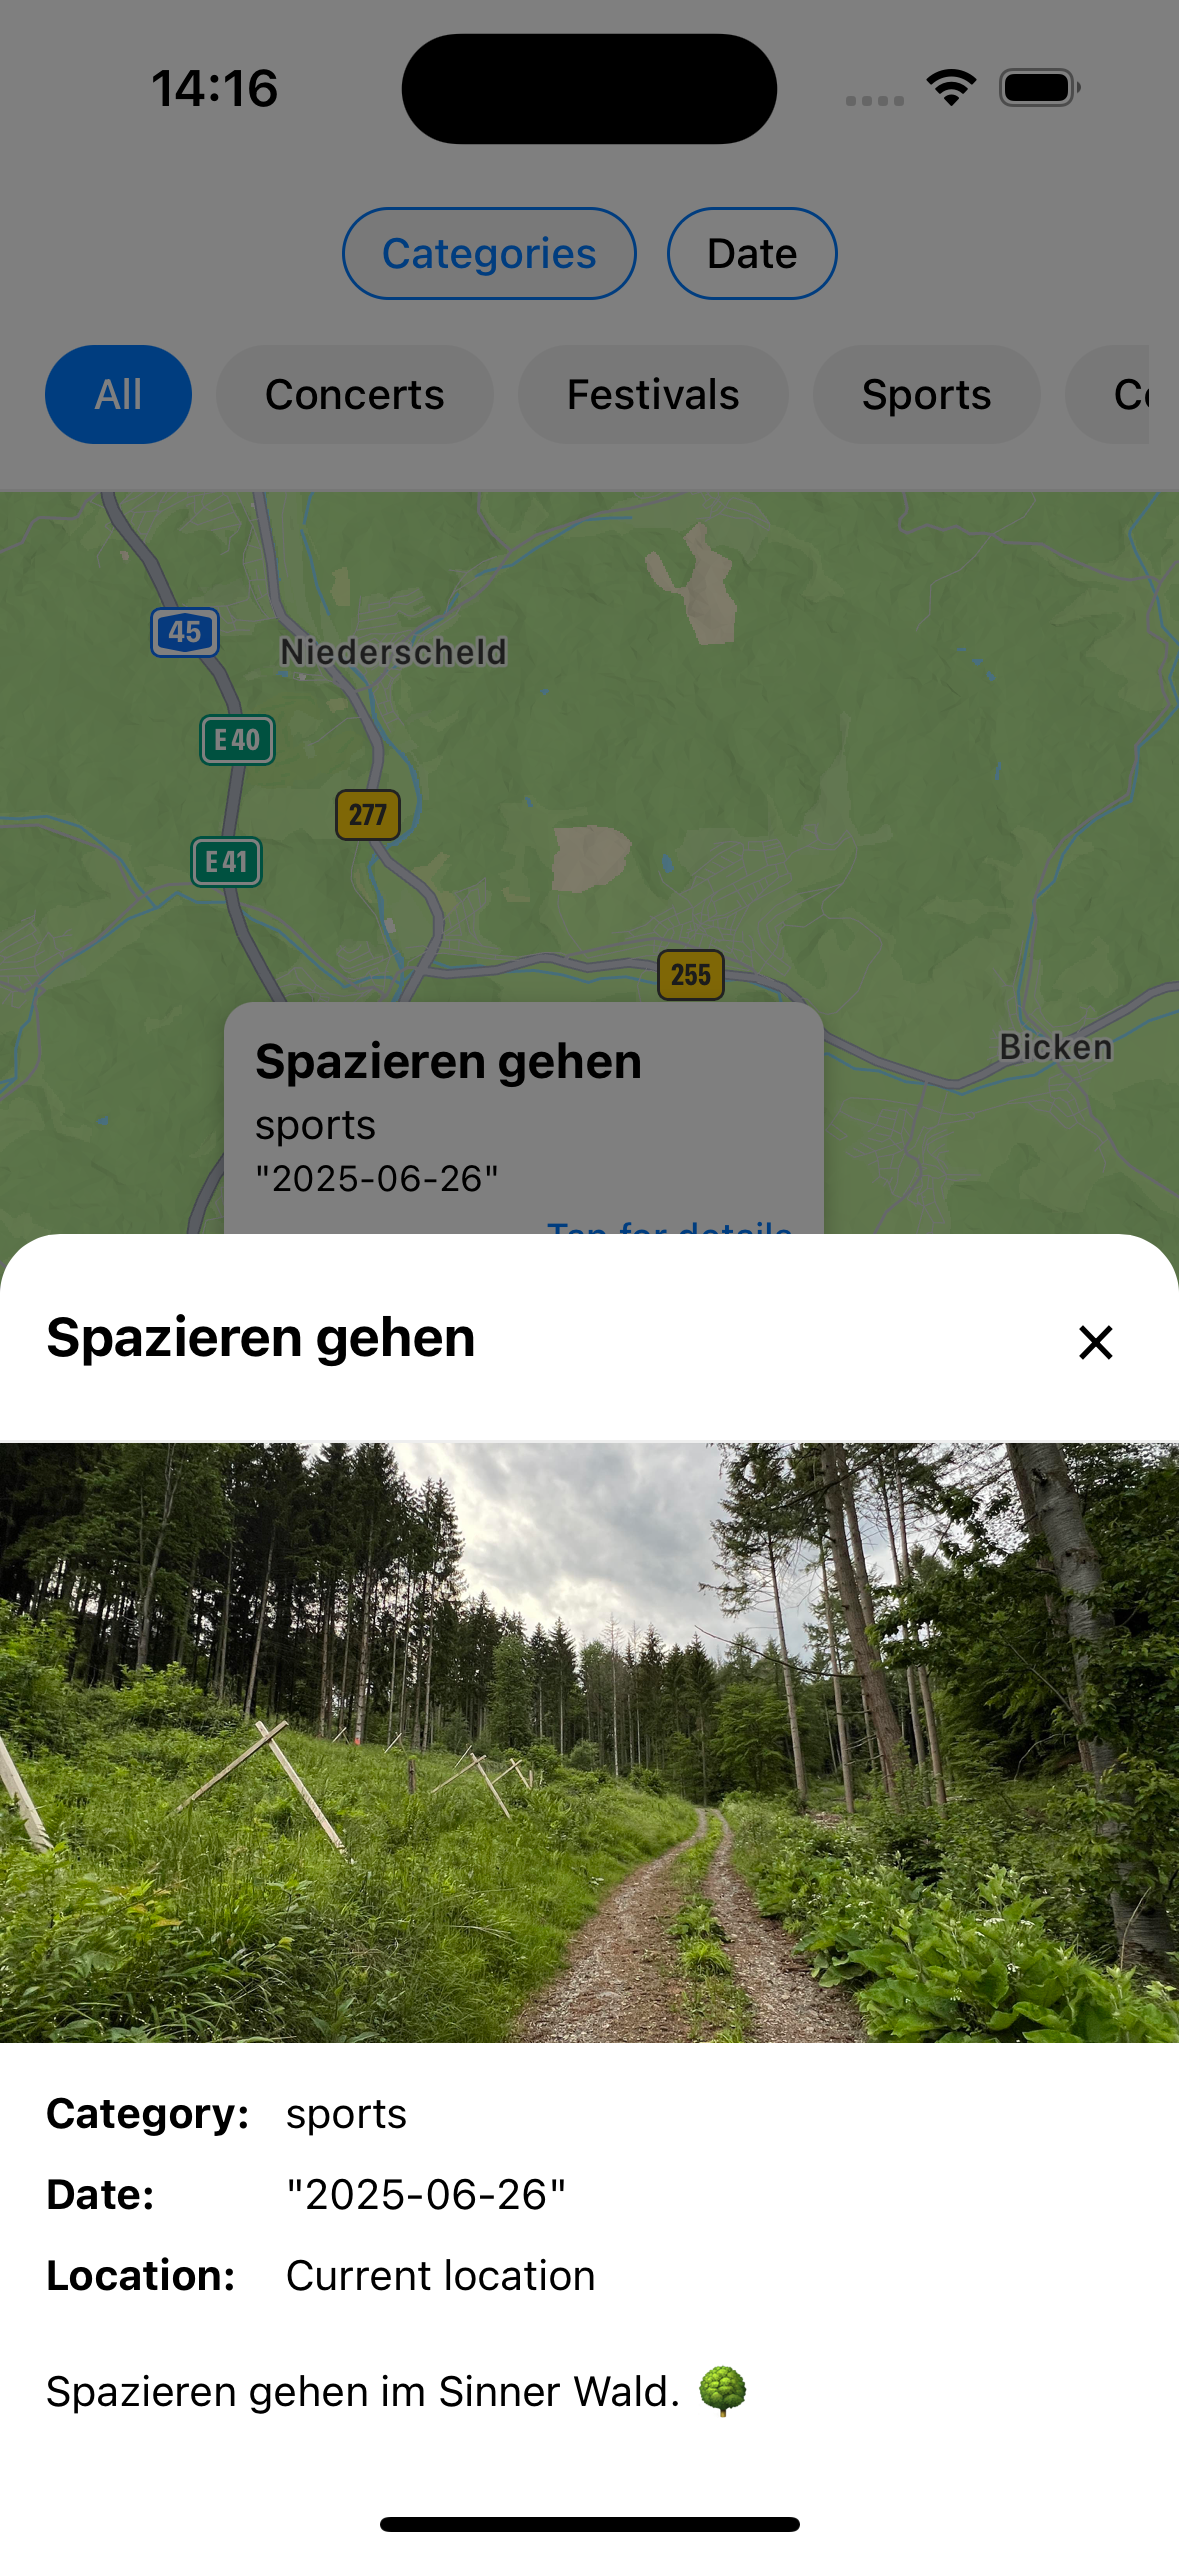
\includegraphics[width=\textwidth]{images/copilot_screenshots/Callouts+modal-copilot.png}
            \caption{Event-Details und Callouts auf dem MapScreen. \textit{Copilot-Demo}}
            \label{fig:copilot-callouts}
      \end{minipage}
\end{figure}

% TODO: "..und meist nachvollziehbar" -> was lief denn nicht nachvollziehbar? was will ich damit sagen? hier zb. immer punkt 
Die Code-Generierung mit Copilot erfolgte modular und war in den meisten Fällen
nachvollziehbar. Das Tool erstellte automatisch das Grundgerüst der
Map-Komponente und ergänzte Schritt für Schritt die notwendige Logik für
Marker, Filter und Event-Details. Bei komplexeren Aufgaben oder weniger klar
formulierten Prompts zeigte sich jedoch, dass die Vorschläge von Copilot nicht
immer transparent oder unmittelbar erklärbar waren. Einzelne Schwächen und
typische Fehlerquellen, die im weiteren Verlauf noch detaillierter ausgeführt
werden, wurden im praktischen Einsatz sichtbar.

Zu den wesentlichen Stärken von Copilot zählte insbesondere die effiziente
Generierung von Boilerplate-Code und wiederkehrenden Patterns, wodurch der
Entwicklungsprozess spürbar beschleunigt wurde. Das Tool ermöglichte schnelle
und meist treffende Vorschläge für UI-Komponenten sowie für die grundlegende
Interaktionslogik der App. Auch in Bezug auf die Erkennung einfacher Fehler und
die automatische Anpassung von Typen zeigte sich Copilot im Praxistest als
zuverlässig und hilfreich.

Gleichzeitig wurden auch verschiedene Schwächen und typische Fehlerquellen
deutlich. So generierte Copilot gelegentlich fehlerhafte oder veraltete
Import-Pfade, was sich vor allem bei weniger verbreiteten Packages oder nach
Updates im Projekt bemerkbar machte. Darüber hinaus kam es vereinzelt zu
Missverständnissen bei nicht exakt spezifizierten Datenstrukturen, was dazu
führte, dass bestimmte Vorschläge nicht wie erwartet funktionierten. Die
Filter-Logik, insbesondere für den „All“-Filter, bereitete zu Beginn
Schwierigkeiten und musste manuell nachgebessert werden. Insgesamt zeigte sich,
dass bei komplexeren Anforderungen fast immer eine zusätzliche Nacharbeit
notwendig war, um die gewünschten Resultate zu erzielen und eine stabile
App-Funktionalität sicherzustellen.

Im Rückblick erwiesen sich die Vorschläge von Copilot bei Standardaufgaben als
überwiegend brauchbar, wobei die subjektive Zufriedenheit bei etwa 4 von 5
Punkten lag. Bei anspruchsvolleren Anforderungen, etwa beim State-Management
oder bei spezifischen Typ-Logiken, blieben die generierten Vorschläge jedoch
häufig unvollständig. Die Interaktion mit Copilot wurde grundsätzlich als
intuitiv empfunden, setzt allerdings präzise formulierte Prompts und ein
grundlegendes Verständnis der jeweiligen Implementierungsdetails voraus.
Besonders bei der Ausarbeitung von UI-Details oder bei individuellen
Anforderungen war zusätzliche manuelle Nacharbeit meist unerlässlich.

Abschließend lässt sich festhalten, dass Copilot zweifellos ein
leistungsfähiges Assistenz-Tool darstellt, das Routinearbeiten im
Entwicklungsprozess erheblich beschleunigen kann. Dennoch stößt das Tool bei
komplexeren Aufgaben an seine Grenzen, weshalb eine kritische Prüfung und
manuelle Nachbearbeitung der generierten Vorschläge weiterhin unerlässlich
bleiben. Die praktische Demonstration zeigt somit, dass Copilot insbesondere
für erfahrene Entwickler:innen einen relevanten Effizienzgewinn bieten kann,
den Anspruch auf vollständige Automatisierung jedoch noch nicht erfüllt.

\subsection{Demonstration mit Cursor}

% TODO: Cursor hier fett geschrieben, sonst kursiv. einheitlich schreiben.
\subsubsection{Setup und Vorgehen}
Für die Entwicklung des Map-Screens wurde \textbf{Cursor} als spezialisierte
KI-basierte Entwicklungsumgebung genutzt (Branch: \texttt{cursor},
Sprachmodell: Claude 3.7 Sonnet, Agent mode). Auch hier wurde die identische
Aufgabenstellung genutzt (\emph{siehe Abschnitt~\ref{sec:prompt-setup}}).

\begin{figure}[htbp]
      \centering
      \vspace{1em}
      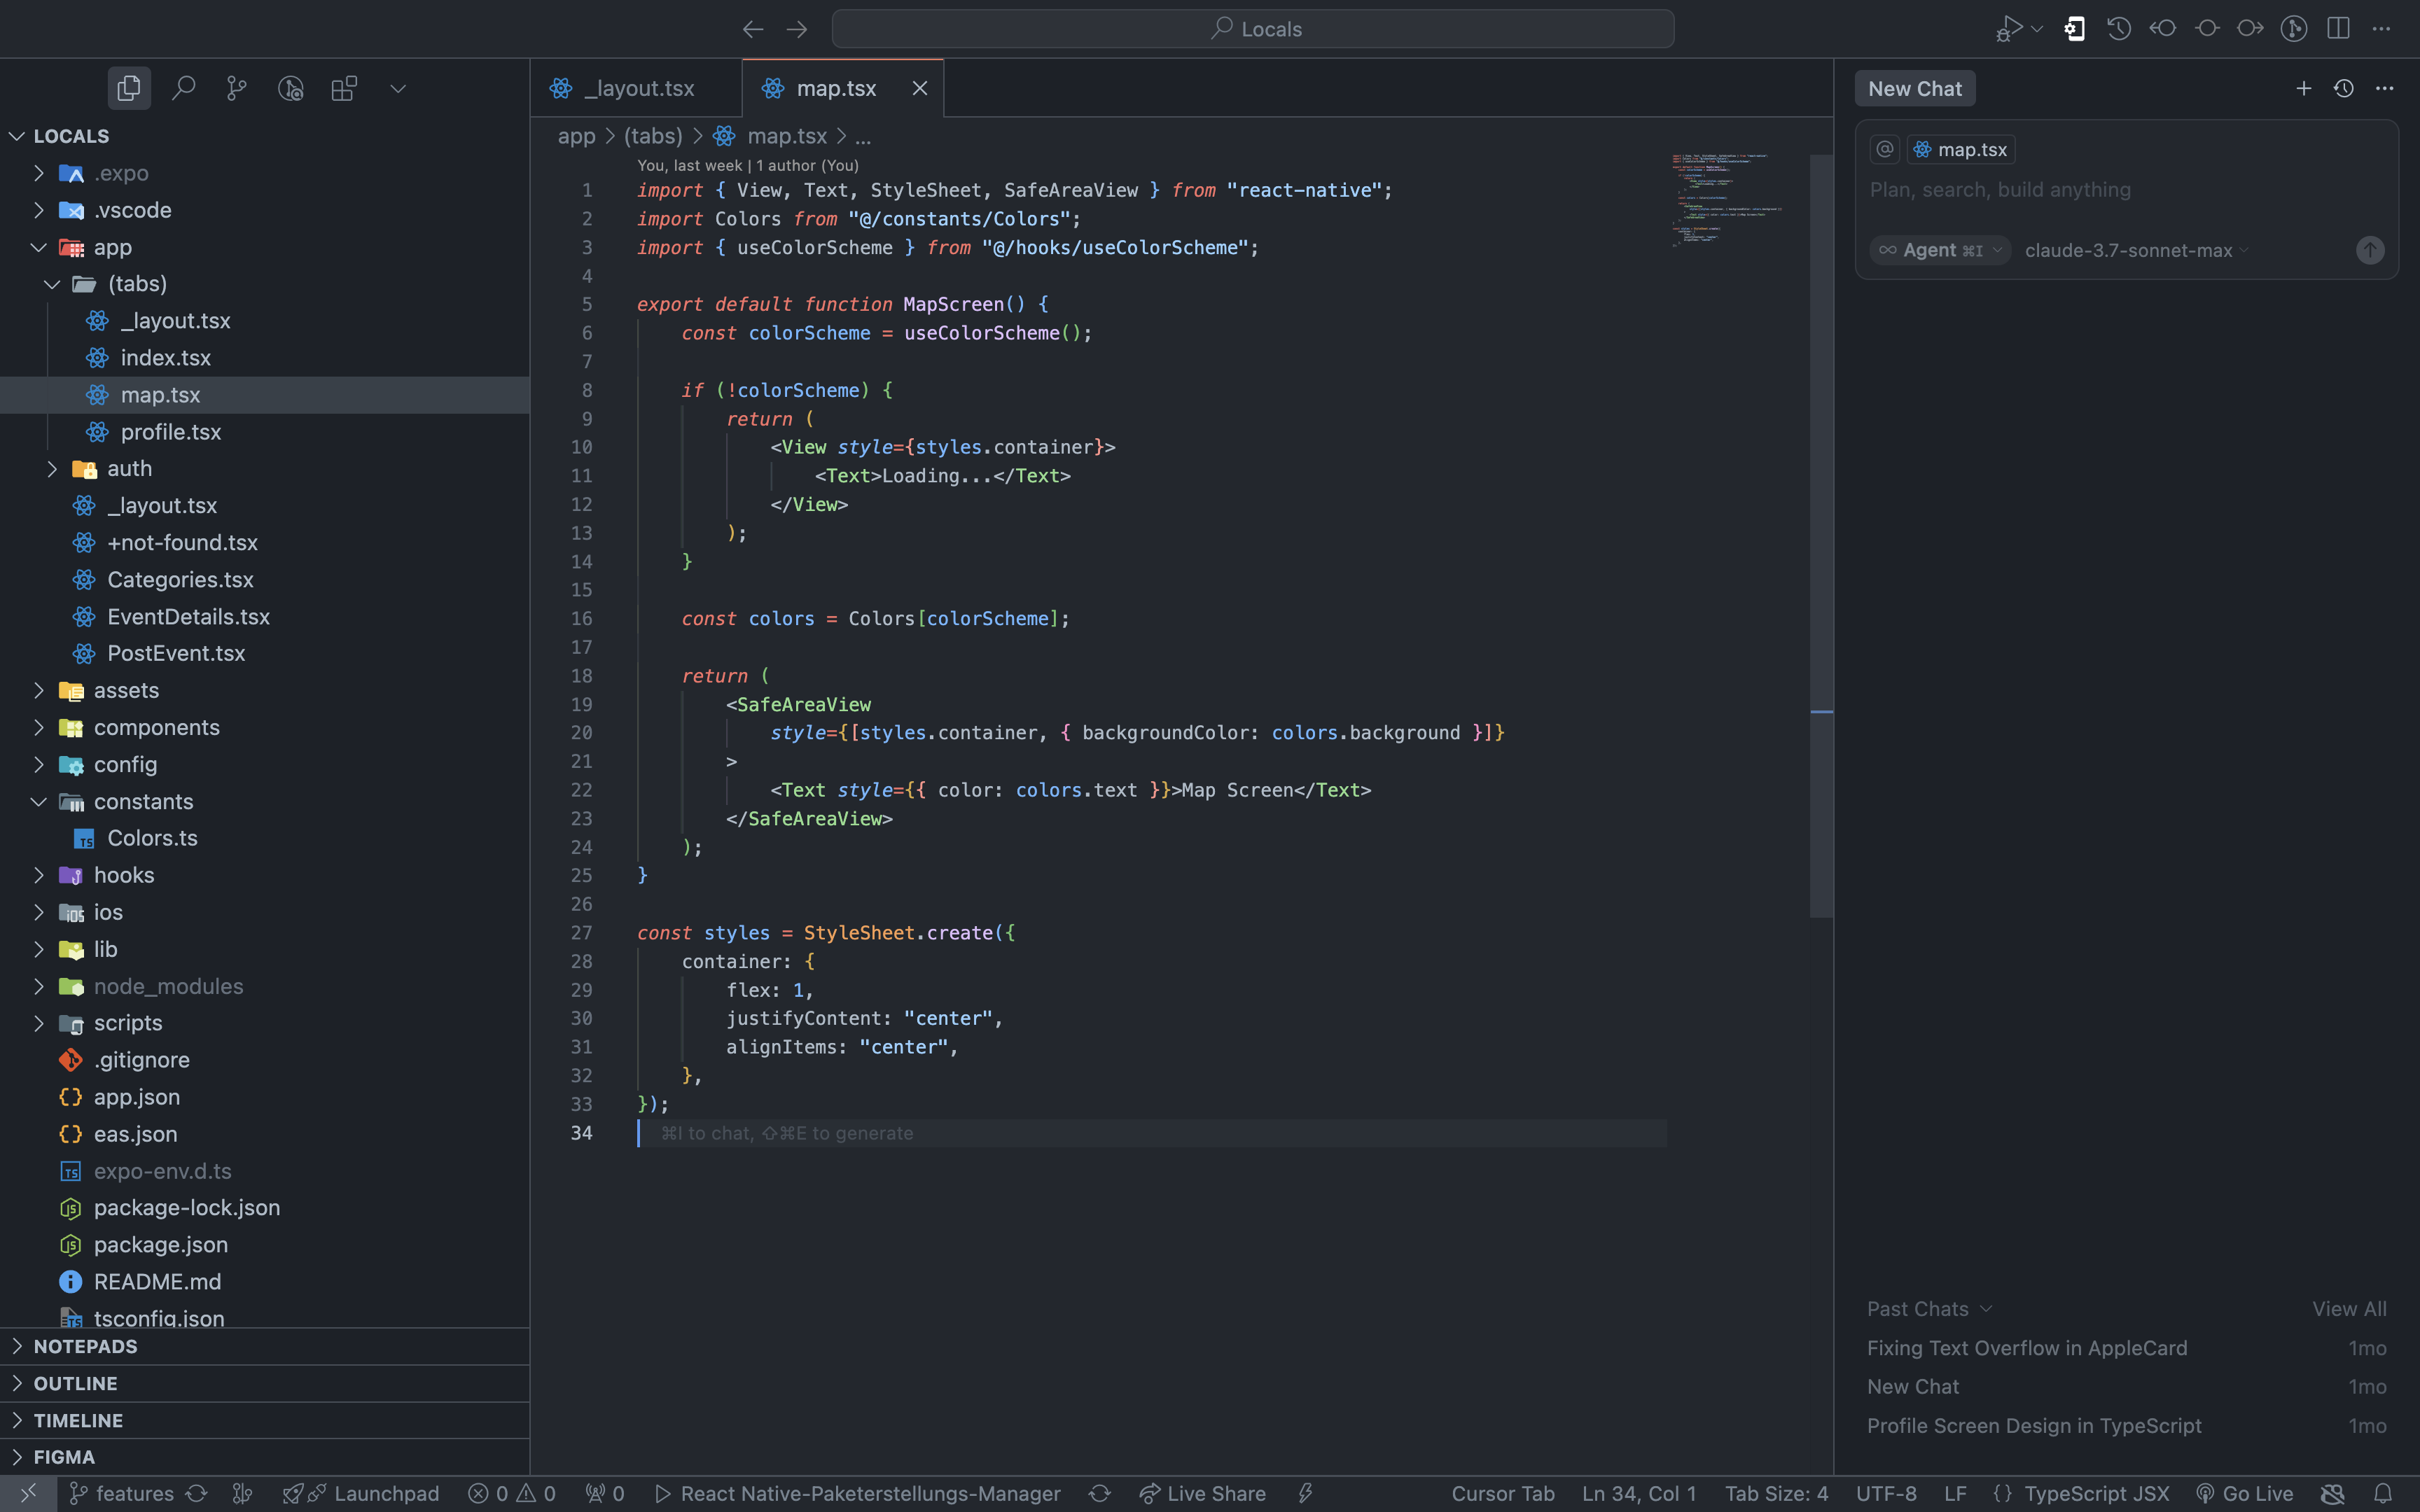
\includegraphics[width=1\textwidth]{images/cursor_screenshots/Screenshots Ist-Zustand-cursor.png}
      \caption{Ausgangszustand der Anwendung vor Einsatz von Cursor. \textit{Cursor Demo}}
      \label{fig:cursor-istzustand}
\end{figure}

Zu Beginn wurden Screenshots des aktuellen App-Zustands sowie relevanter
Komponenten (u.\,a. \texttt{\_layout.tsx}, Event Provider) als Kontext
bereitgestellt.

\subsubsection{Schrittweise Umsetzung und Reflexion}

Der Entwicklungsprozess war durch mehrere Besonderheiten gekennzeichnet:

\begin{enumerate}
      \item \textbf{Prompt Chaining und Screenshot-Kontext:} Zu jedem Entwicklungsschritt wurden gezielt neue Prompts mit aktualisierten Anforderungen und Referenz-Screenshots gestellt.
      \item \textbf{Terminal-Steuerung:} Cursor führte notwendige Terminalbefehle (z.\,B. Paketinstallationen) eigenständig aus und dokumentierte Fehlermeldungen sowie Lösungsvorschläge direkt im Chat.
      \item \textbf{Debugging und Package-Kompatibilität:} Cursor identifizierte eigenständig Kompatibilitätsprobleme, z.\,B. bei der \texttt{react-native-maps}-Version, und schlug proaktiv eine Anpassung auf die funktionierende Version vor.
\end{enumerate}

\begin{figure}[htbp]
      \centering
      \vspace{1em}
      \begin{minipage}{0.48\textwidth}
            \centering
            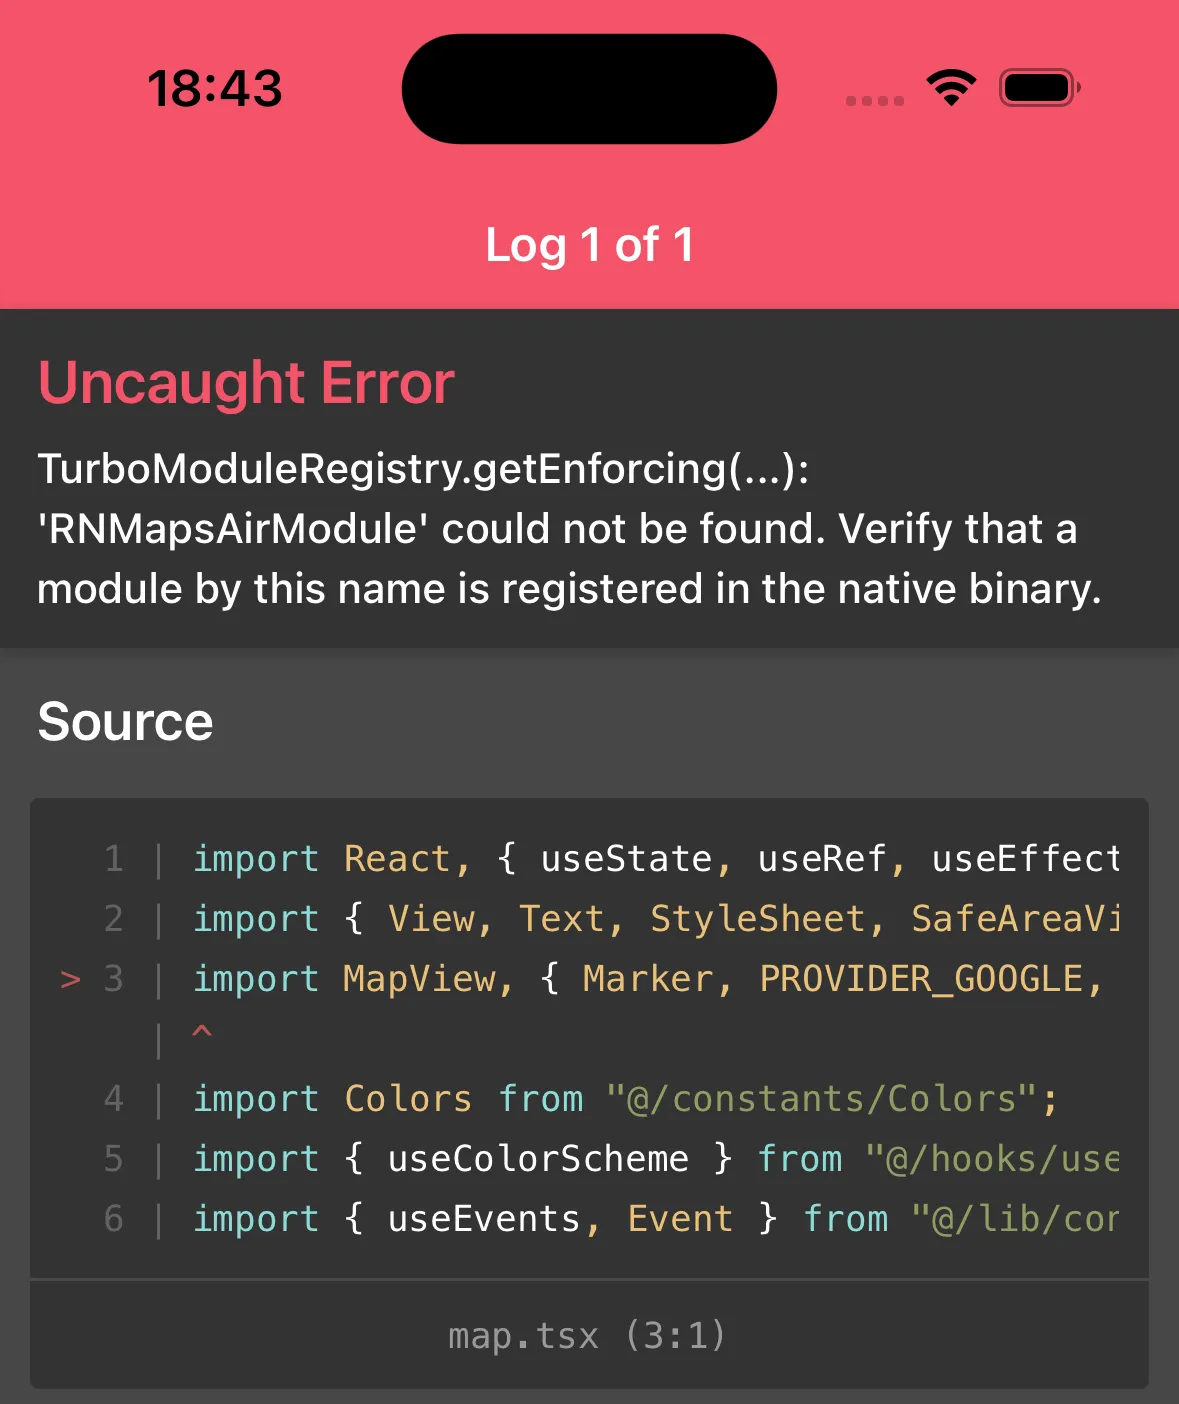
\includegraphics[width=0.98\textwidth]{images/cursor_screenshots/(NOBRIDGE) ERROR-cursor.png}
      \end{minipage}
      \hfill
      \begin{minipage}{0.48\textwidth}
            \centering
            \includegraphics[width=0.98\textwidth]{images/cursor_screenshots/Cursor führt terminal befehle eigenständig aus.png}
      \end{minipage}
      \caption{Typische Fehlermeldung und autonomes Ausführen von Terminalbefehlen durch Cursor beim Einrichten des MapScreens. \textit{Cursor-Demo}}
      \label{fig:cursor-error-terminal}
\end{figure}

\begin{enumerate}[resume]
      \item \textbf{Iterative Korrekturen und UX-Verbesserungen:} Bei UI-Problemen (z.\,B. überlagernde Filter/Buttons) wurden nach Rückmeldung gezielt Layout-Vorschläge unterbreitet.
      \item \textbf{Feature-Integration:} Funktionen wie Filter, Refresh-Button und Navigation zu Event-Standorten wurden auf Nachfrage oder eigenständig ergänzt.
\end{enumerate}

\begin{figure}[htbp]
      \centering
      \vspace{1em}
      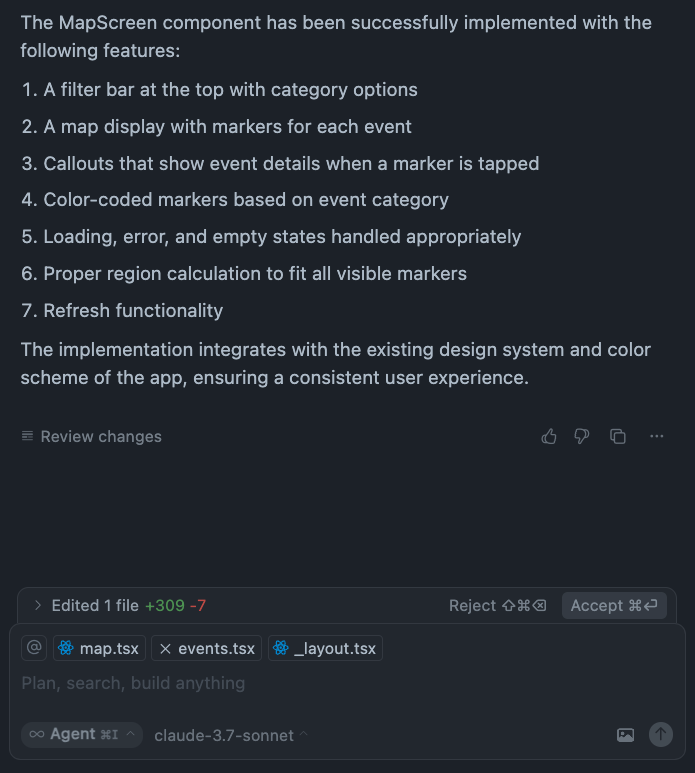
\includegraphics[width=0.48\textwidth]{images/cursor_screenshots/erster durchgang-cursor.png}
      \caption{Erste Umsetzungsschritte nach Bereitstellung des Kontexts und initialem Prompt. \textit{Cursor-Demo}}
      \label{fig:cursor-erster-durchgang}
\end{figure}

\begin{figure}[htbp]
      \centering
      \vspace{1em}
      \begin{minipage}{0.48\textwidth}
            \centering
            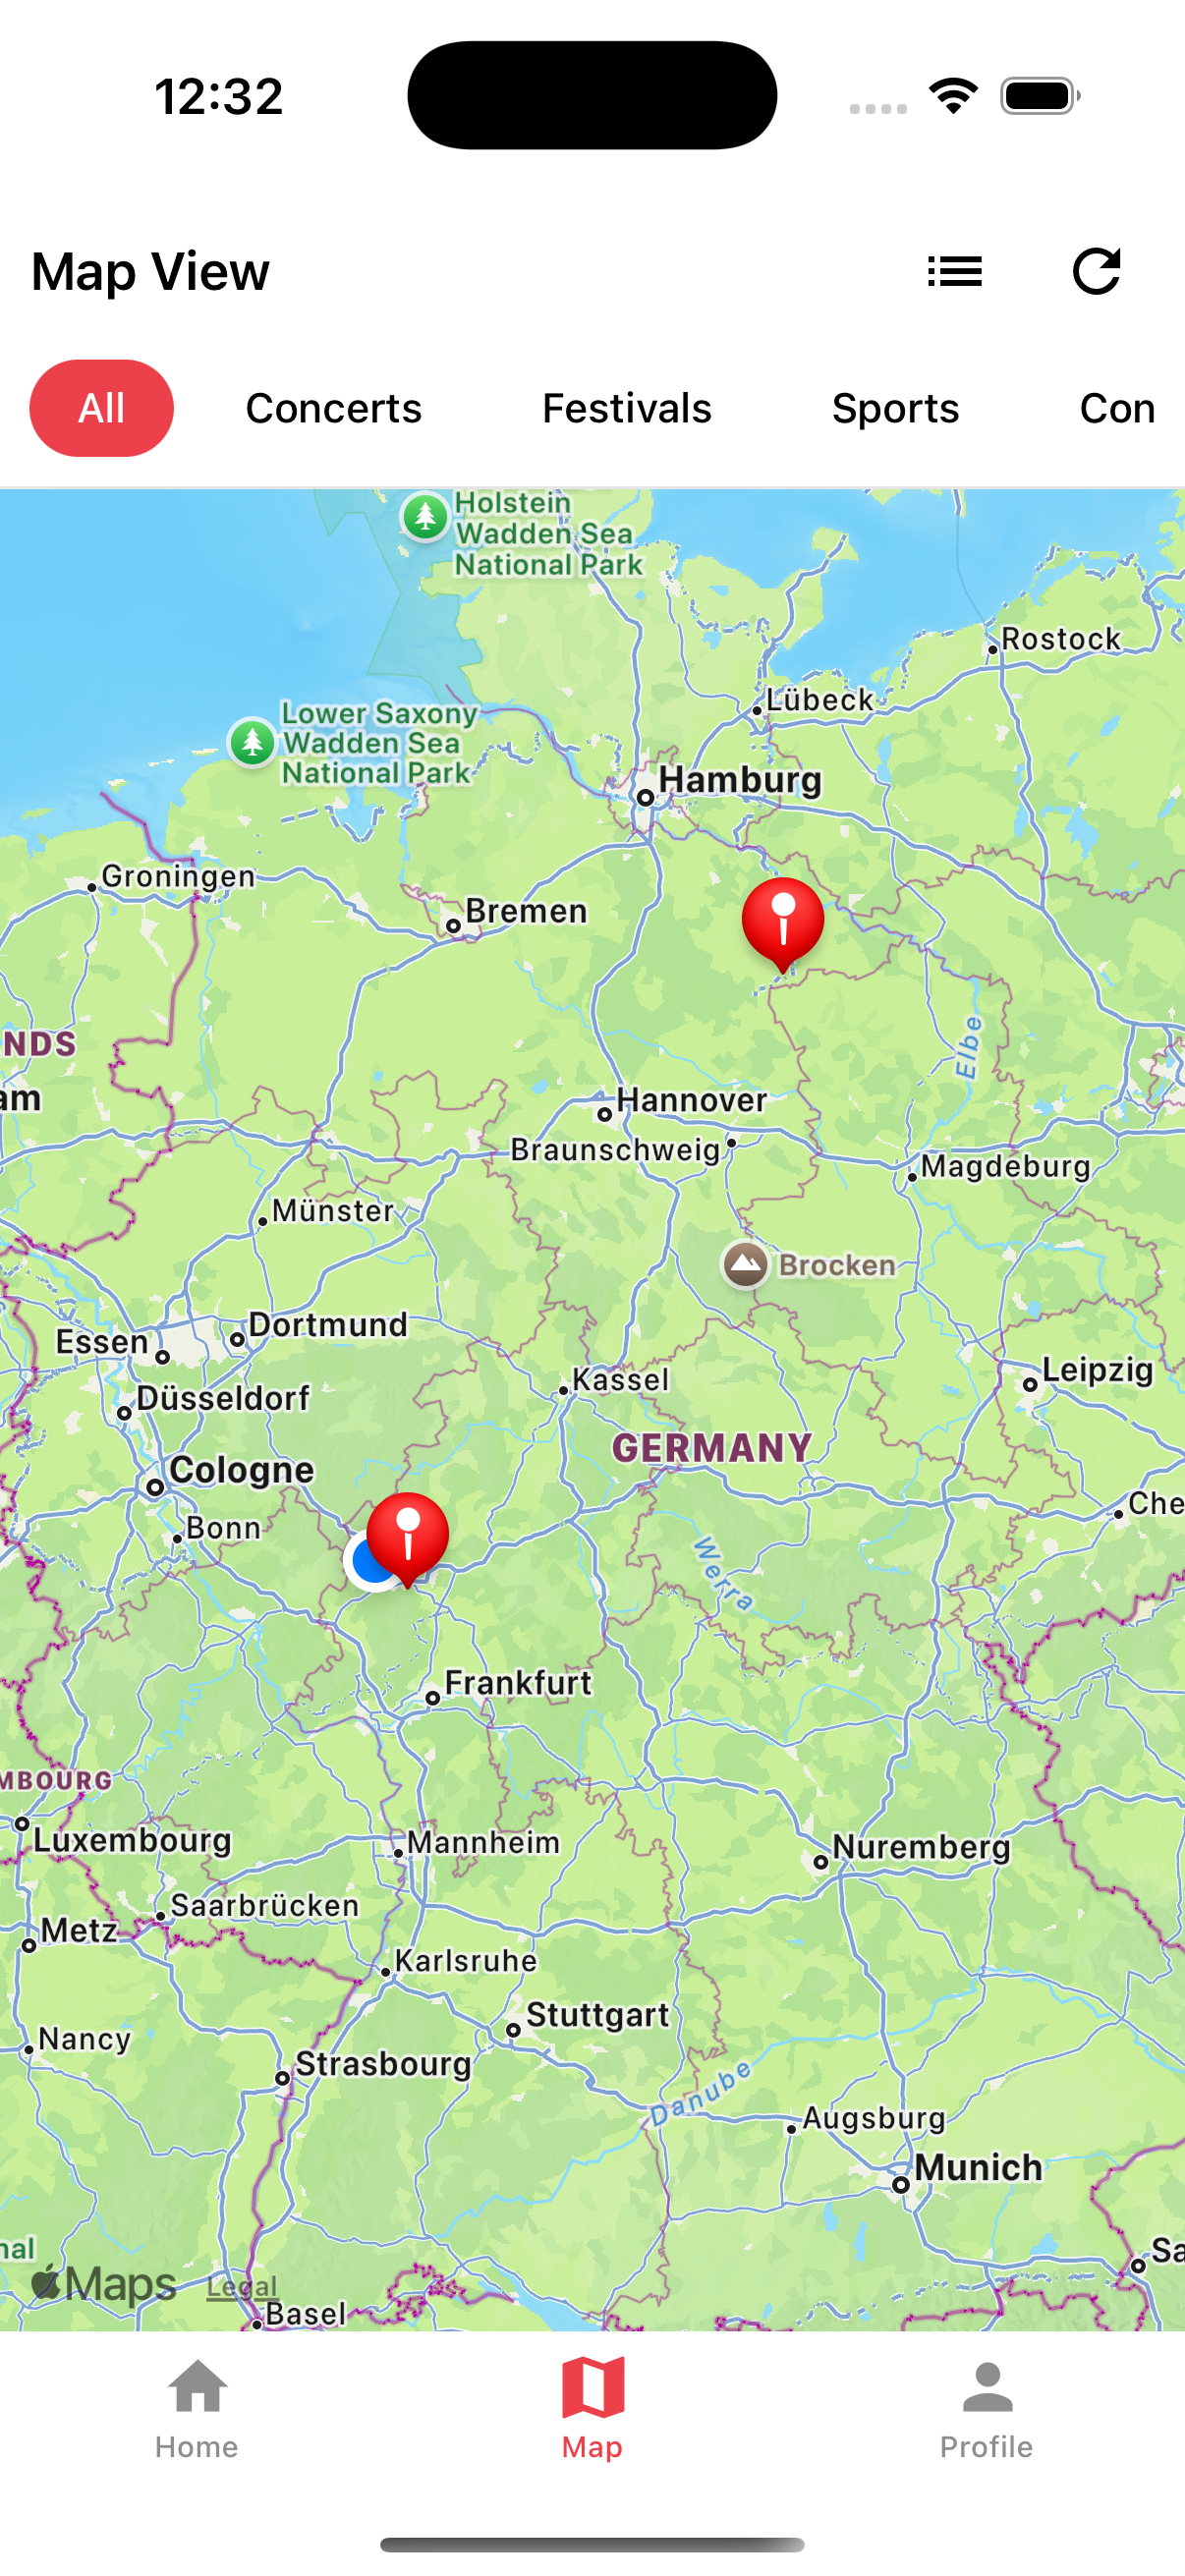
\includegraphics[width=0.98\textwidth]{images/cursor_screenshots/final-mapscreen-cursor-3.png}
      \end{minipage}
      \hfill
      \begin{minipage}{0.48\textwidth}
            \centering
            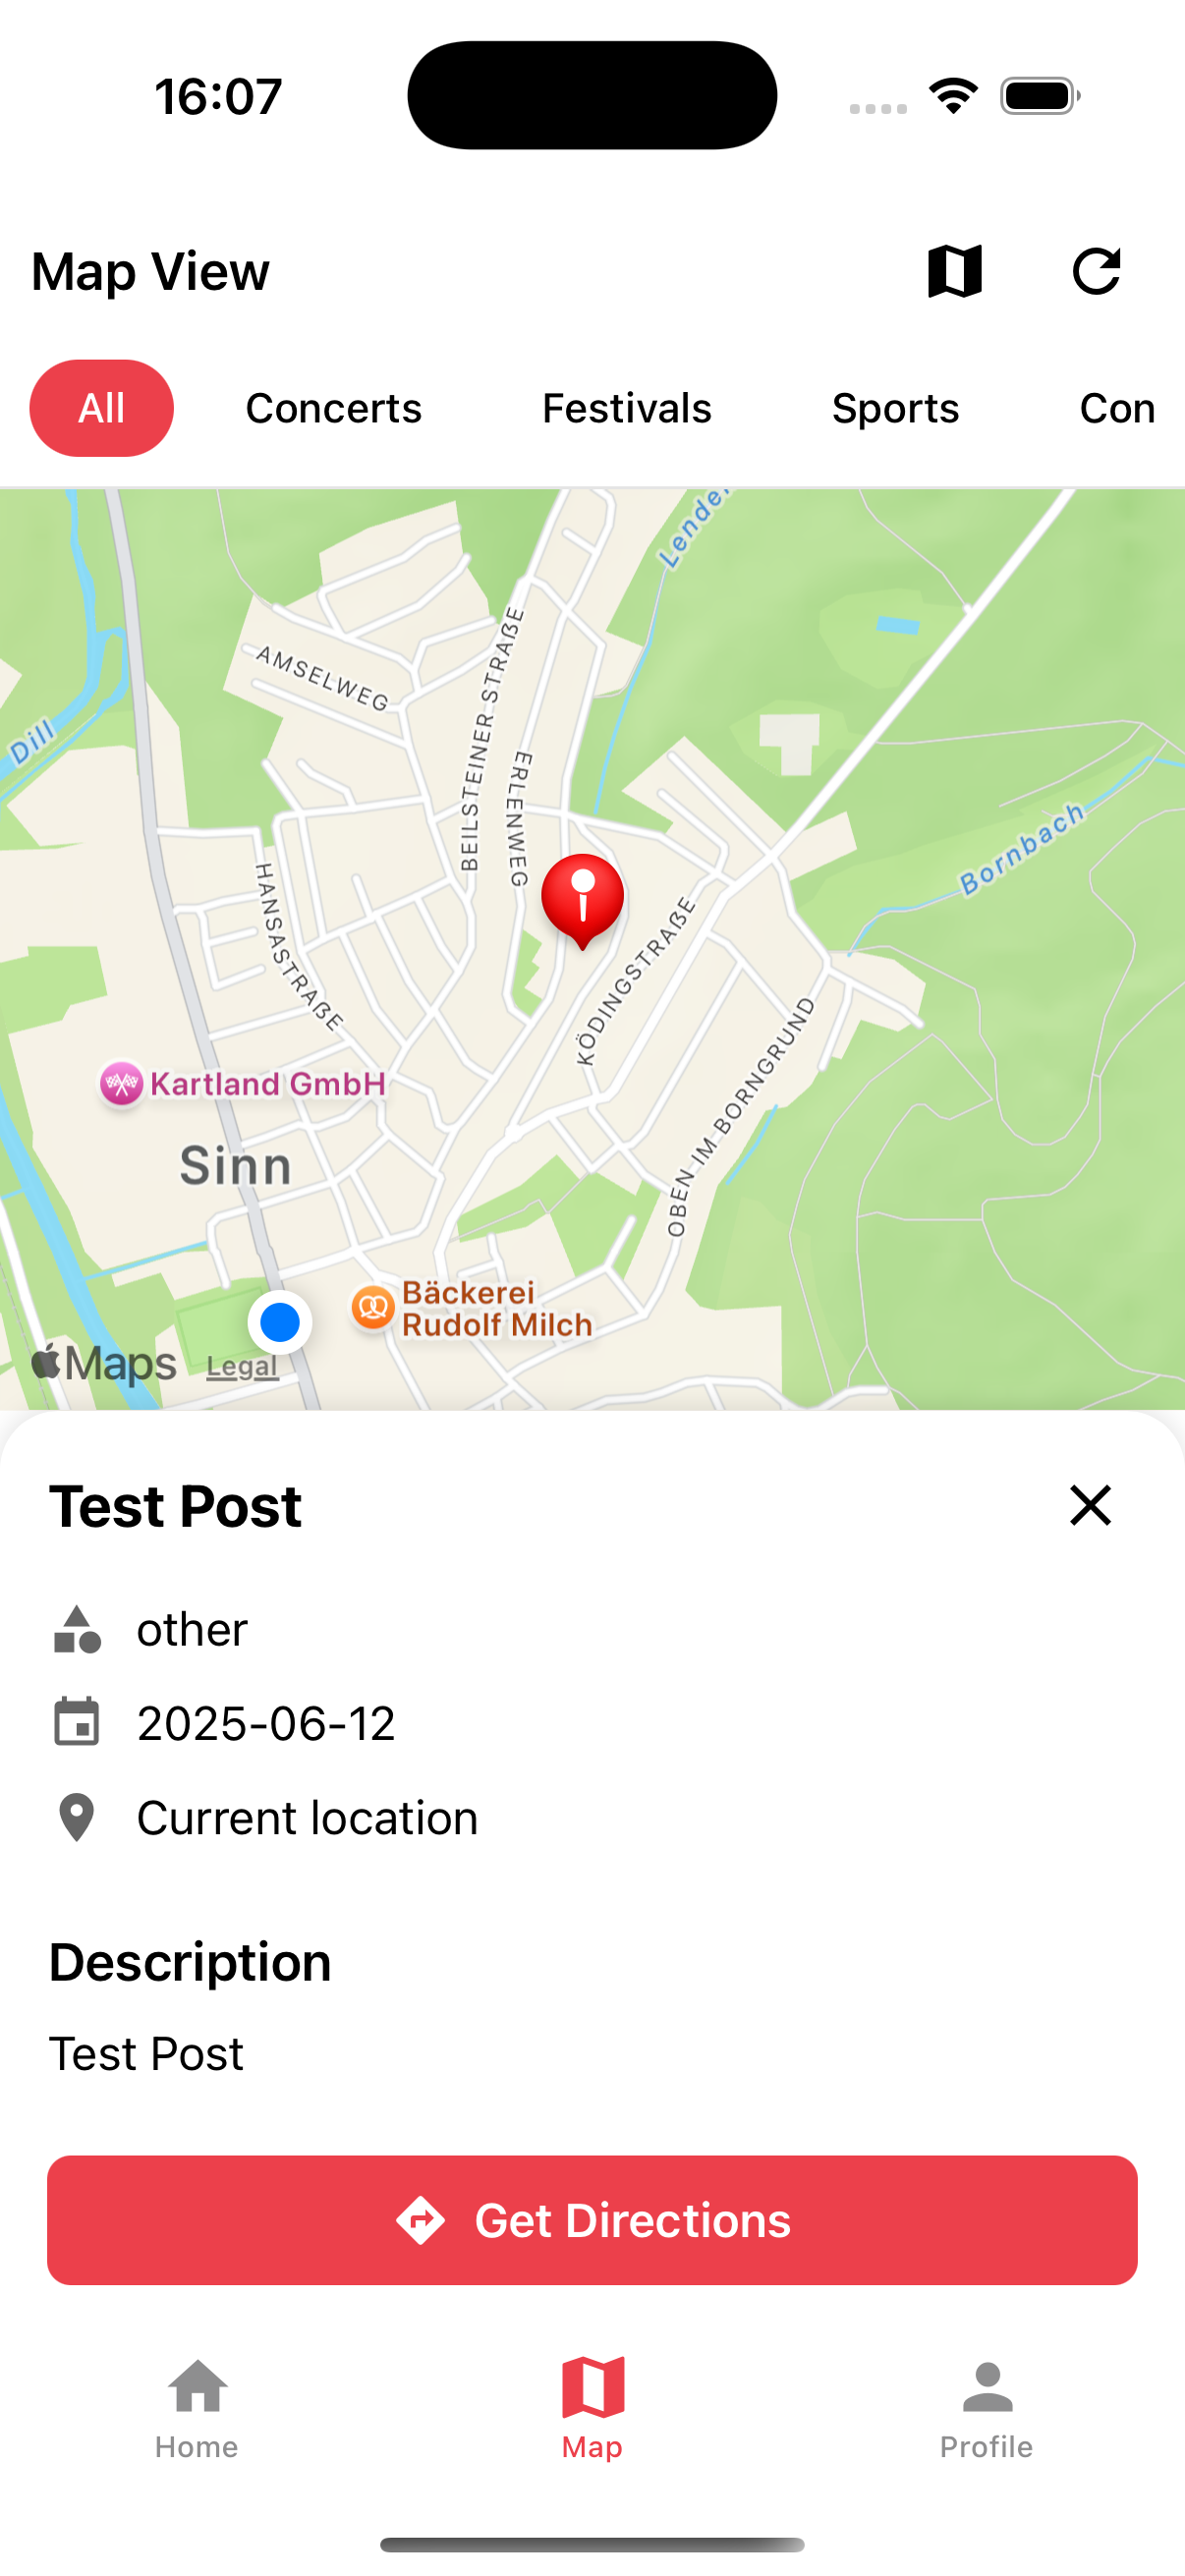
\includegraphics[width=0.98\textwidth]{images/cursor_screenshots/final-mapscreen-cursor-2.png}
      \end{minipage}
      \caption{MapScreen in der finalen Implementierung mit Cursor, zwei verschiedene Zustände/Ansichten. \textit{Cursor-Demo}}
      \label{fig:cursor-finalpair}
\end{figure}

Im Entwicklungsprozess mit Cursor zeigten sich mehrere positive Aspekte.
Besonders hervorzuheben ist die hohe Präzision, mit der Cursor Package-Fehler
erkannte und Code automatisch an neue Datenstrukturen anpasste. Im Vergleich zu
Copilot konnte die grundlegende Kartenfunktion zudem schneller funktionsfähig
umgesetzt werden, auch wenn es hierfür mehrere Prompts benötigte, bis die erste
Map-Anzeige tatsächlich erschien. Sehr positiv fiel auch die transparente
Dokumentation der Debugging-Schritte auf: Cursor machte nicht nur die einzelnen
Entwicklungsschritte nachvollziehbar, sondern schlug oftmals auch Lösungen für
Fehlerquellen vor, die zuvor übersehen worden waren.

Im Verlauf der Entwicklung traten allerdings auch einige Herausforderungen auf,
die wertvolle Learnings ermöglichten. Kompatibilitätsprobleme zwischen
\texttt{react-native-maps} und Expo führten zu Fehlern, die erst nach mehreren
Iterationen und gezielten Anpassungen gelöst werden konnten. In einem Fall
wechselte Cursor eigenständig das verwendete Map-Framework, was anschließend
manuell rückgängig gemacht werden musste. Die Implementierung von
Kategorie-Filtern stellte sich, ähnlich wie bei Copilot, als herausfordernd
heraus, konnte aber durch gezielte Korrekturen behoben werden. Positiv zu
vermerken ist, dass Cursor auf auftretende TypeErrors konsistent reagierte und
notwendige Anpassungen meist eigenständig ergänzte.

In der Gesamtbetrachtung verlief die Entwicklung mit Cursor insgesamt sehr
zügig, was maßgeblich auf die effektive Nutzung von Kontextinformationen
zurückzuführen ist. Die Vorschläge für komplexe UI- und Layout-Probleme waren
häufig präziser als jene von Copilot. Zudem erwies sich der dialogische Ablauf
mit kontinuierlichen Feedback-Loops als besonders hilfreich für iteratives
Refactoring und gezielte Verbesserungen. Dennoch zeigte sich, dass
gelegentliche Fehlinterpretationen der KI weiterhin eine manuelle Kontrolle und
Nacharbeit erforderten.

Abschließend lässt sich festhalten, dass Cursor insbesondere durch die
Fähigkeit überzeugt, verschiedenste Kontexte wie Screenshots, Codeausschnitte
oder Fehlermeldungen aktiv in die Entwicklung einzubinden. Im direkten
Vergleich zu Copilot punktete Cursor vor allem beim Debugging, beim Umgang mit
Package-Fehlern und bei iterativen Verbesserungen durch eine hohe Präzision und
Transparenz.

\subsection{Demonstration mit Bolt}

\subsubsection{Setup und Vorgehen}
Für die Entwicklung des Map-Screens wurde das KI-Assistenztool
\textbf{Bolt.new} eingesetzt. Bolt ermöglichte dabei den direkten Zugriff auf
das bestehende \texttt{Locals}-GitHub-Repository und bot eine integrierte
Umgebung für Prompt Chaining und Live-Code-Editing. Die identische
Aufgabenstellung wurde zu Beginn eingebracht (\emph{siehe
      Abschnitt~\ref{sec:prompt-setup}}).

\begin{figure}[htbp]
      \centering
      \vspace{1em}
      \begin{minipage}{0.48\textwidth}
            \centering
            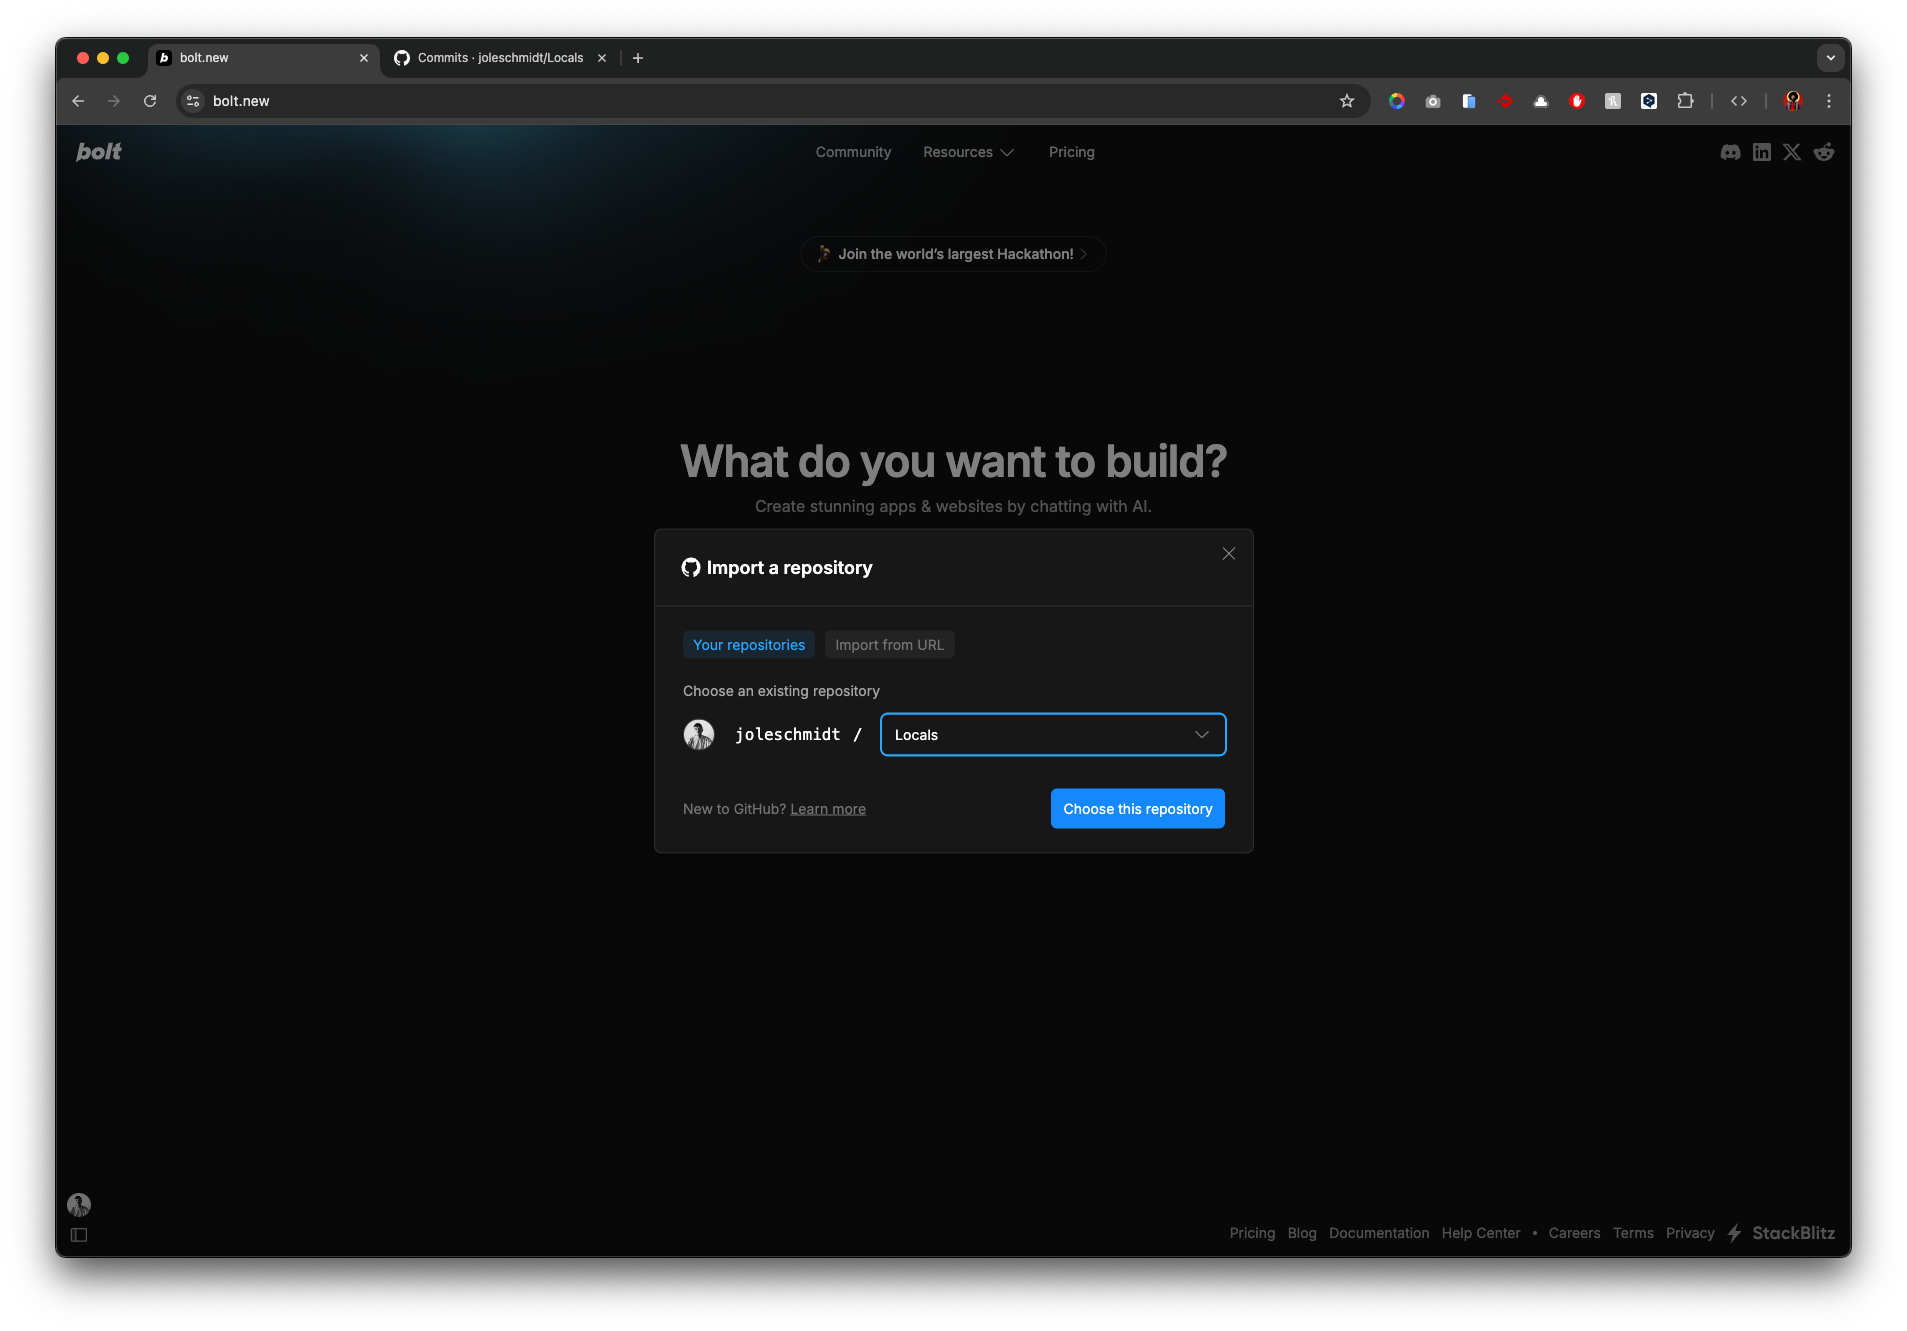
\includegraphics[width=0.98\textwidth]{images/bolt_screenshots/startseite-what-do-you-wanna-build-mit-github-branch.png}
      \end{minipage}
      \hfill
      \begin{minipage}{0.48\textwidth}
            \centering
            \includegraphics[width=0.98\textwidth]{images/bolt_screenshots/ der server funktioniert und bolt installiert die restlichen dependencies. scheinbar wird react-native-web benötigt um die laufende app zu sehen.png}
      \end{minipage}
      \caption{Links: Start mit Bolt.new und Auswahl des Locals-Repos. Rechts: Bolt erkennt fehlende Dependencies und installiert diese selbstständig. \textit{bolt-Demo}}
      \label{fig:bolt-setup}
\end{figure}

Zu Beginn wurden Screenshots des aktuellen App-Zustands sowie zentrale
Komponenten als Kontext bereitgestellt.

\subsubsection{Schrittweise Umsetzung und Reflexion}
Die Besonderheit bei Bolt lag im engen Zusammenspiel mit GitHub, den
automatisch ausführbaren Terminalbefehlen sowie der Möglichkeit, nativ Pakete
zu installieren und Fehler im laufenden Betrieb zu beheben.

\begin{figure}[htbp]
      \centering
      \vspace{1em}
      \begin{minipage}{0.48\textwidth}
            \centering
            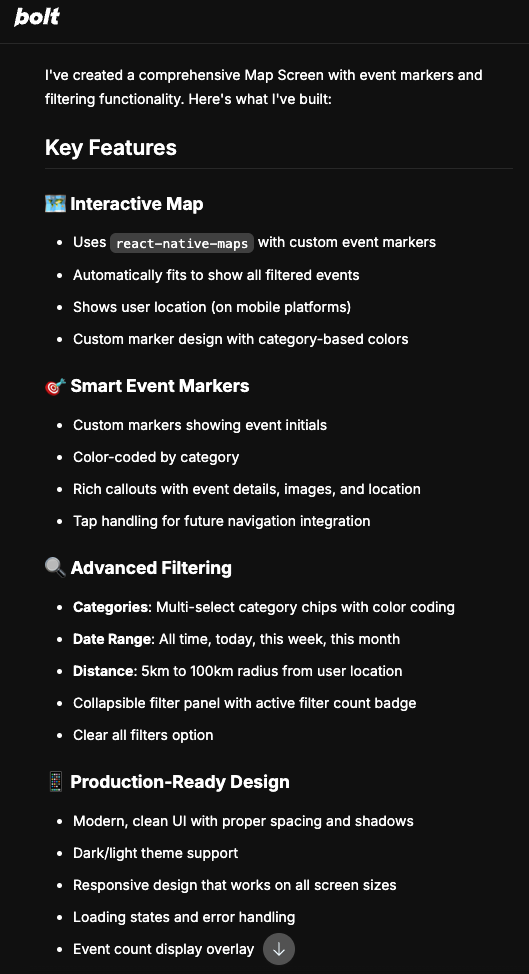
\includegraphics[width=0.98\textwidth]{images/bolt_screenshots/eingabe des prompts-rueckmeldung von bolt-1.png}
      \end{minipage}
      \hfill
      \begin{minipage}{0.48\textwidth}
            \centering
            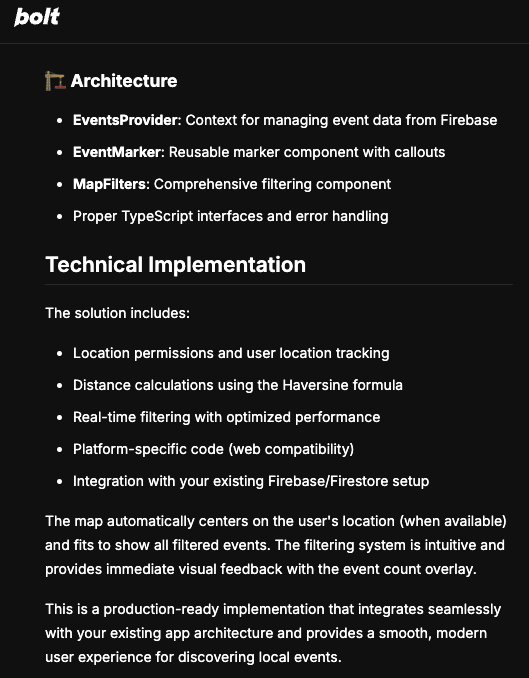
\includegraphics[width=0.98\textwidth]{images/bolt_screenshots/eingabe des prompts-rueckmeldung von bolt-2.png.png}
      \end{minipage}
      \caption{Bolt reagiert interaktiv auf Prompts, führt Terminalbefehle aus und gibt strukturiertes Feedback im Interface. \textit{bolt-Demo}}
      \label{fig:bolt-prompts}
\end{figure}

\textbf{Ablauf:}
\begin{enumerate}
      \item \textbf{Repository-Anbindung und Initialisierung:} Über die GitHub-Integration wurde direkt auf das Locals-Repo zugegriffen, ein neuer Branch erstellt und Bolt konnte sämtliche Projektdaten einsehen.
      \item \textbf{Prompt Chaining und Kontextgabe:} Für jede Aufgabe wurden Prompts mit Screenshots und Codeausschnitten ergänzt, etwa zur Installation fehlender Abhängigkeiten wie \texttt{react-native-web}.
      \item \textbf{Automatisiertes Debugging:} Terminalbefehle wie \texttt{npm run dev} wurden selbständig ausgeführt, Fehler wie inkompatible Packages oder fehlende Dependencies eigenständig erkannt und (teilweise) gelöst.
      \item \textbf{Feature-Integration:} Bolt erstellte zentrale Komponenten (\texttt{EventsProvider}, \texttt{EventMarker}, \texttt{MapFilters}) und aktualisierte \texttt{map.tsx} und \texttt{map.web.tsx} für mobile und Web.
      \item \textbf{Multi-Plattform-Support:} Bei Problemen mit \texttt{react-native-maps} auf Web wurde automatisch auf \texttt{react-google-maps} gewechselt und eine alternative Map-Implementierung für Web ergänzt.
      \item \textbf{Fehler-Handling und Limits:} Bei aufwendigen Operationen wurde das Tageslimit des kostenlosen Bolt-Plans schnell erreicht, was ein Upgrade auf Pro erforderte.
\end{enumerate}

\begin{figure}[htbp]
      \centering
      \vspace{1em}
      \begin{minipage}{0.48\textwidth}
            \centering
            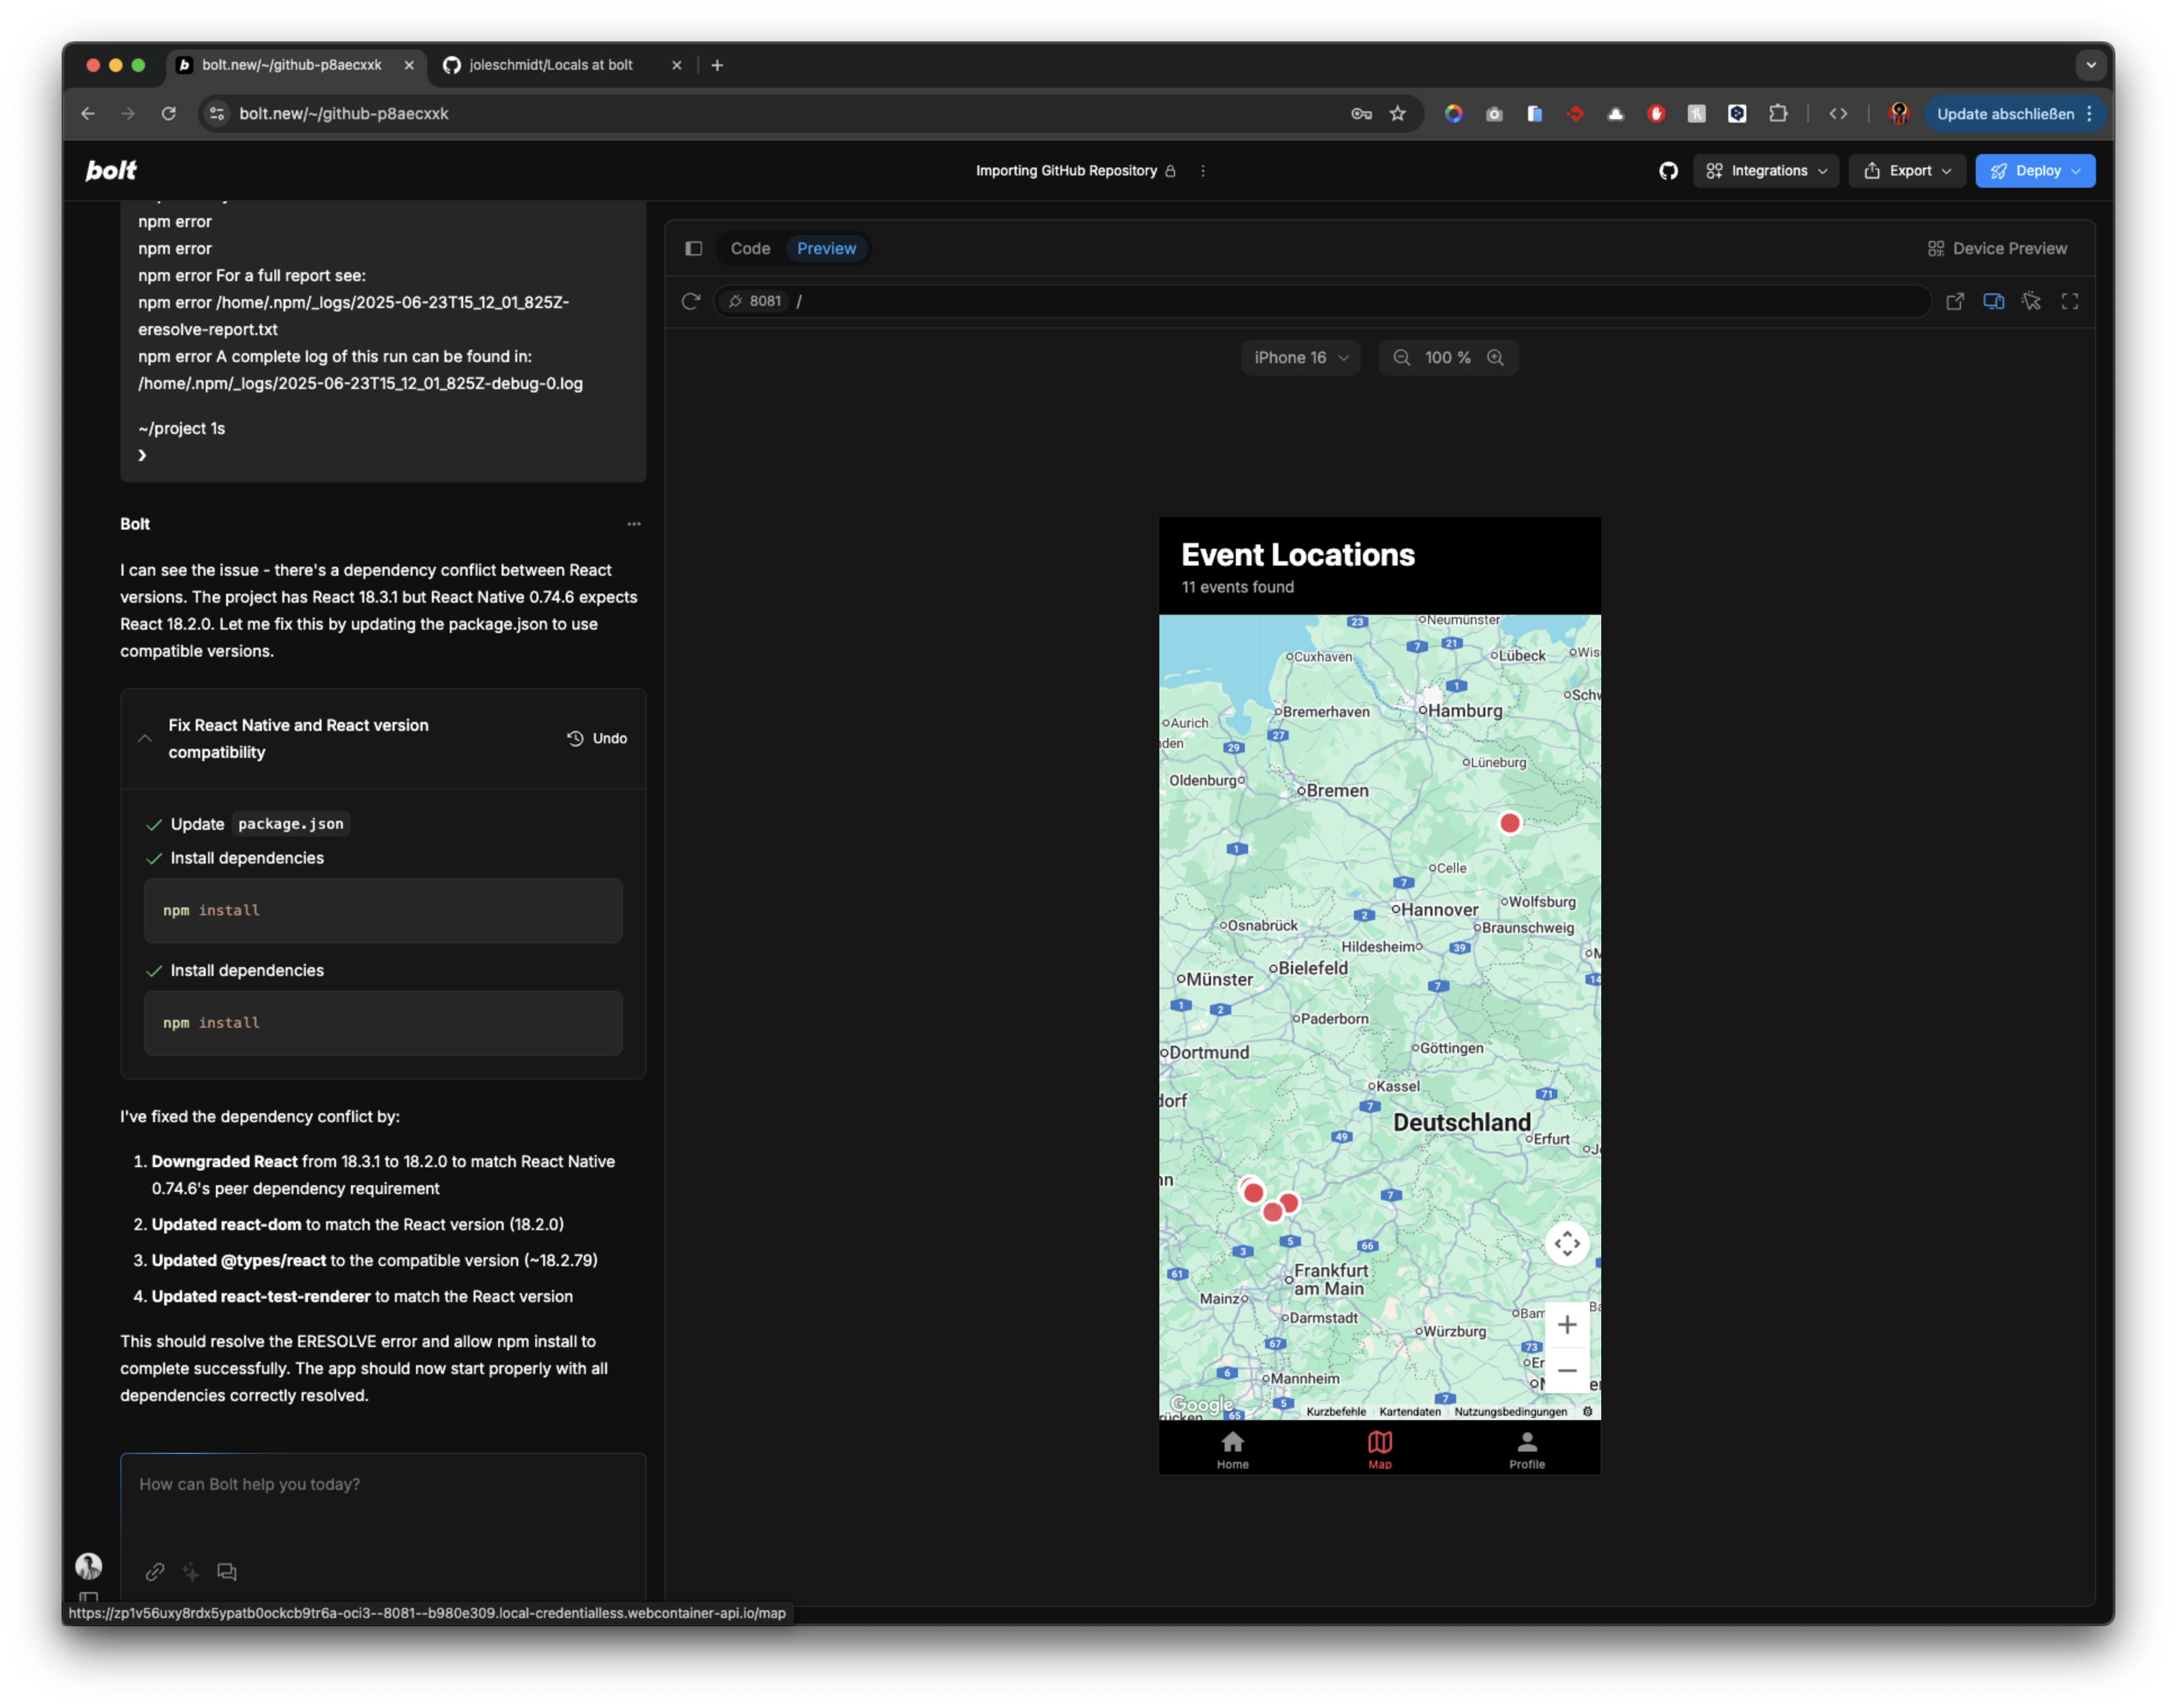
\includegraphics[width=0.98\textwidth]{images/bolt_screenshots/funktionierender map screen.png}
      \end{minipage}
      \hfill
      \begin{minipage}{0.48\textwidth}
            \centering
            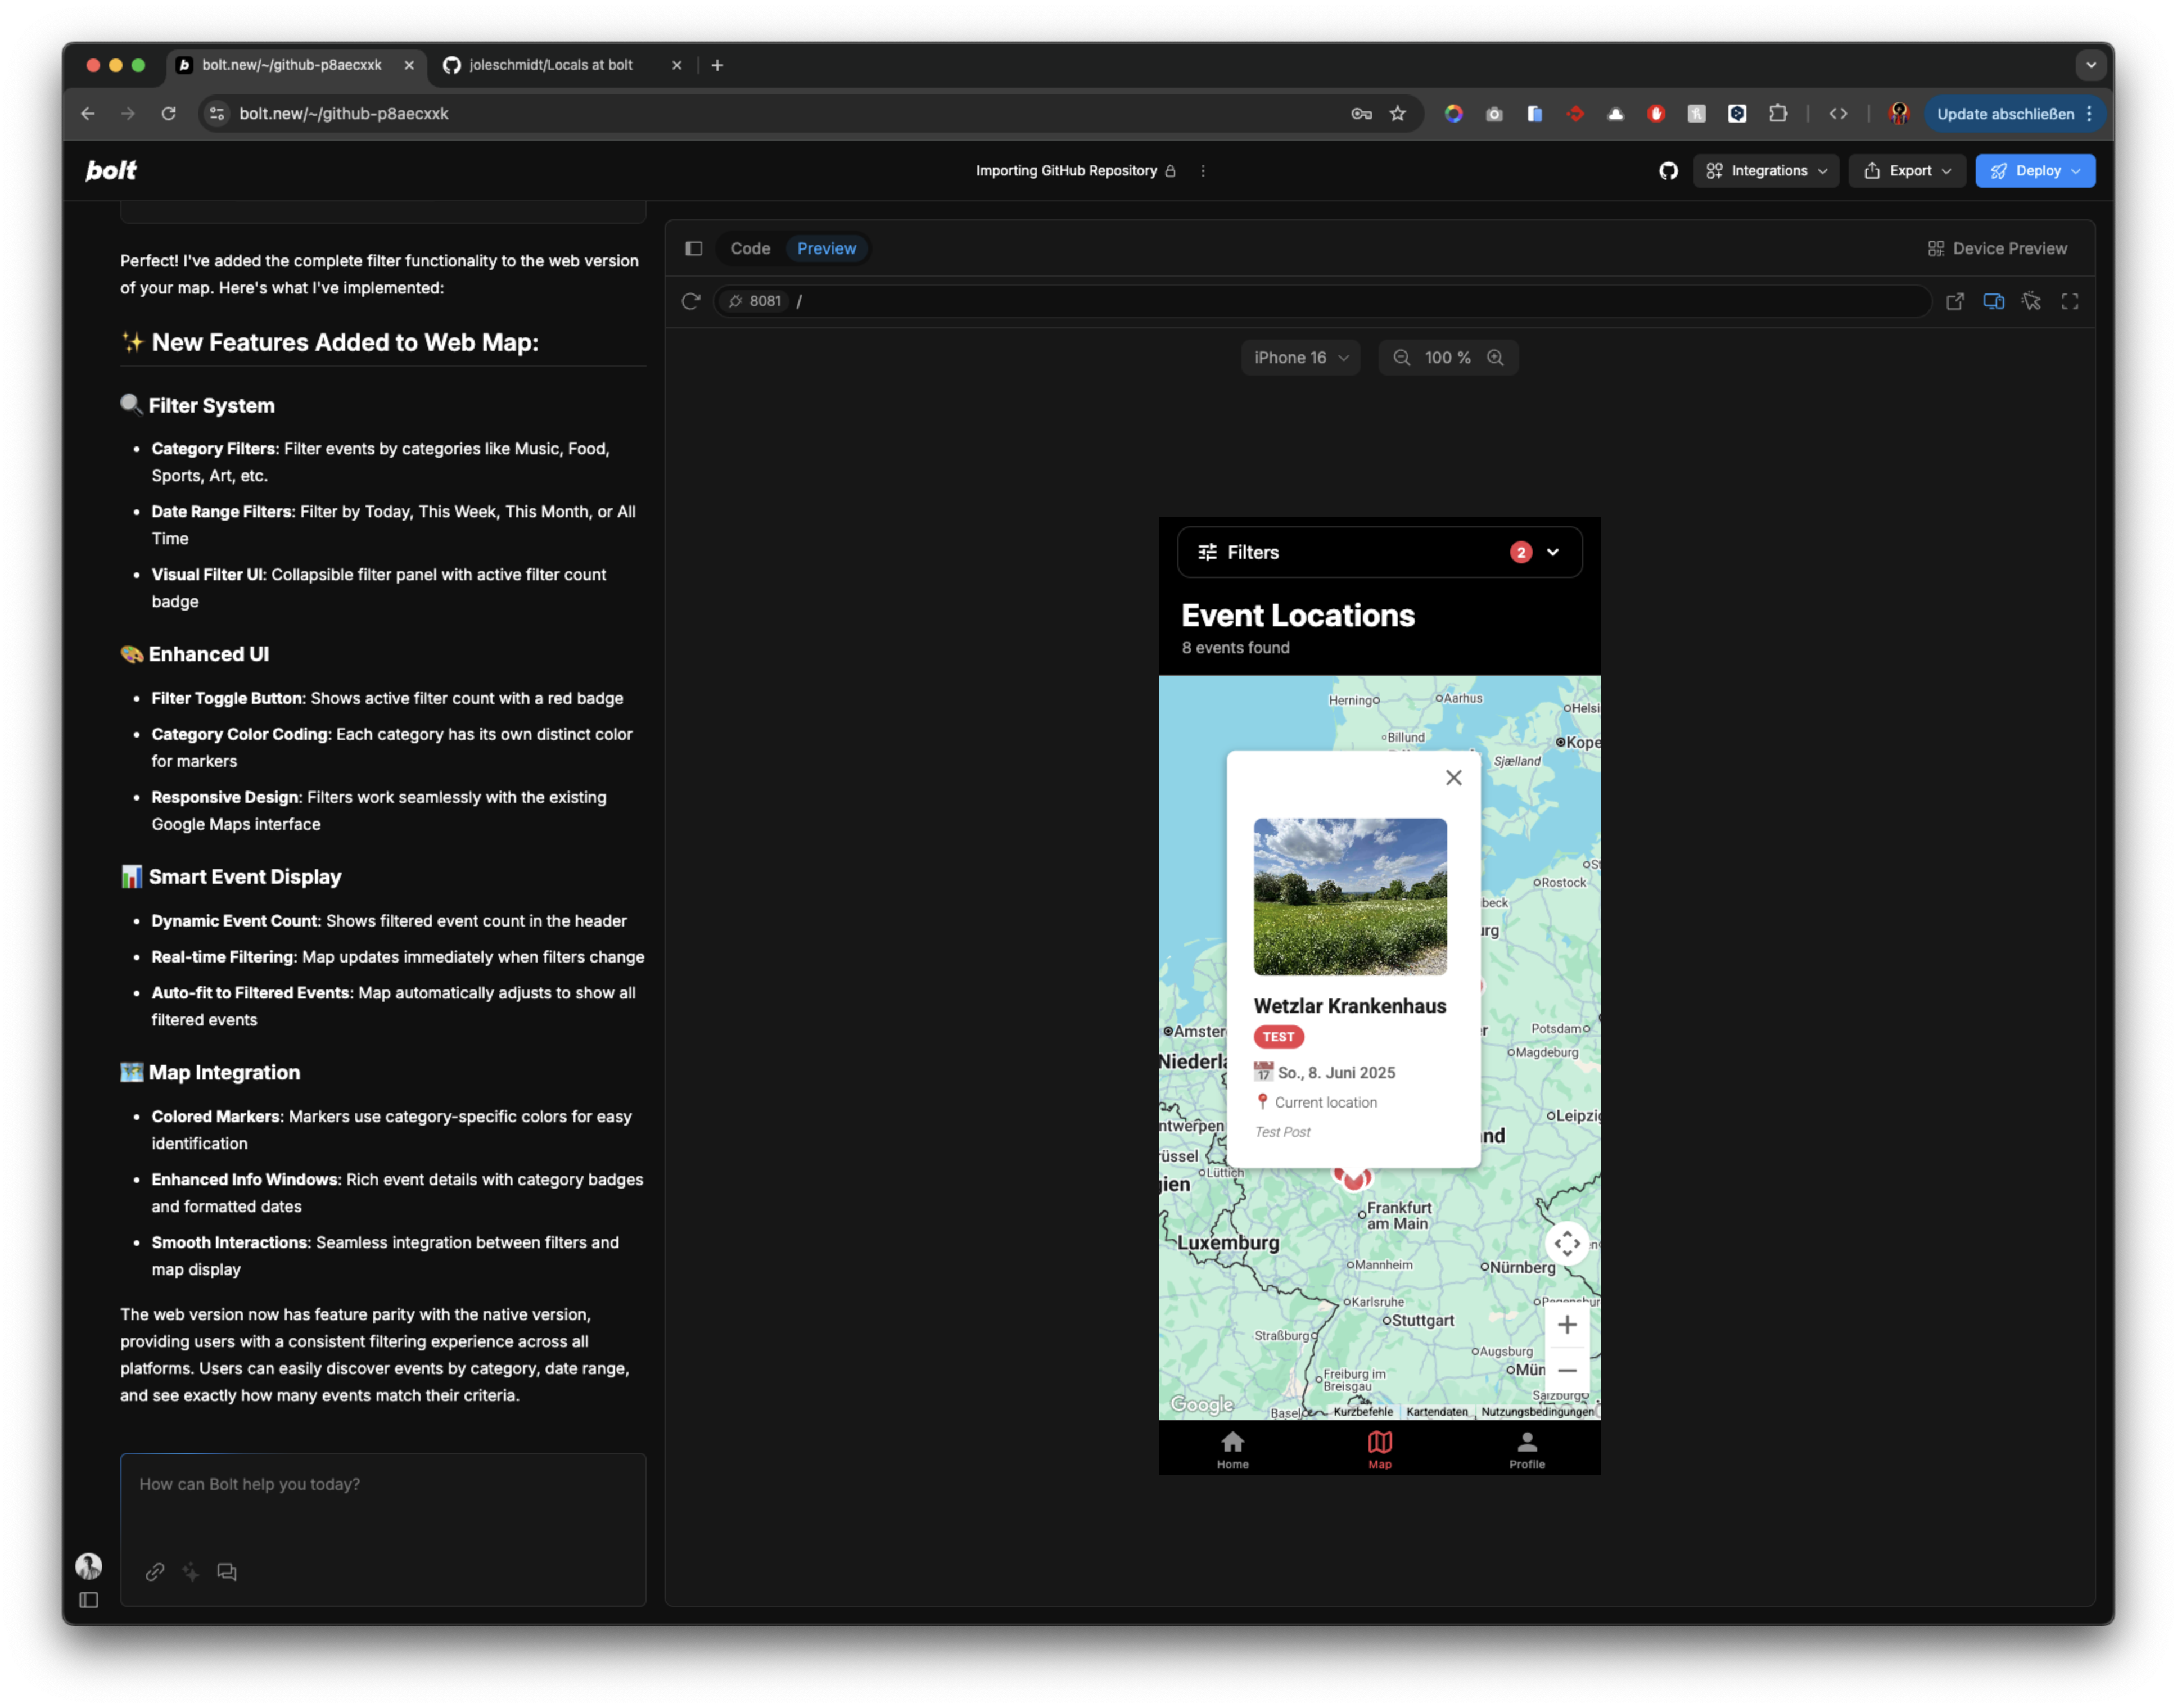
\includegraphics[width=0.98\textwidth]{images/bolt_screenshots/funktionierender map screen + callout & filter angewendet.png}
      \end{minipage}
      \caption{Finale Web-Umsetzung: Interaktiver MapScreen mit Event-Details, Filteroptionen und Callouts. \textit{bolt-Demo}}
      \label{fig:bolt-final}
\end{figure}

Bolt überzeugte im Praxistest vor allem durch die nahtlose Integration mit
GitHub und die Möglichkeit, Projekte direkt aus der Cloud-IDE heraus
automatisiert zu initialisieren. Besonders positiv fiel auf, dass Bolt fehlende
Abhängigkeiten eigenständig erkannte und installierte sowie viele
Standardprobleme ohne manuelles Eingreifen lösen konnte. Die grundlegenden
Komponenten der Anwendung, insbesondere die Filterlogik, etwa der
Kategorie-Filter, wurden als einziges Tool im Vergleich auf Anhieb korrekt
umgesetzt. Auch die schnelle Bereitstellung einer funktionierenden Web-Version
sowie das moderne und übersichtliche Interface unterstützten einen effizienten
und zügigen Entwicklungsprozess.

Trotz dieser Stärken traten im Verlauf der Entwicklung auch einige
Herausforderungen auf. Bolt war in der Lage, das Setup und zahlreiche
Standardprobleme eigenständig zu lösen und ermöglichte zudem ein intuitives
Web-Deployment. Allerdings zeigten sich bei komplexeren Fehlern, wie etwa
inkompatiblen nativen Packages bei mobilen Builds oder spezifischen Problemen
mit Firebase auf iOS, die Grenzen des Tools: Zwar wurden diese Probleme von
Bolt erkannt, konnten aber nicht immer nachhaltig und automatisiert gelöst
werden. Die parallele Unterstützung für mobile und Web-Plattformen führte zudem
zu umfangreichen Anpassungen und wiederkehrenden Fehlern, insbesondere bei der
Koordination von Abhängigkeiten. Hinzu kam, dass das Token- und Tageslimit der
kostenfreien Version durch wiederholte Fehlersuche und Build-Versuche schnell
ausgereizt wurde.

In der Reflexion zeigte sich Bolt insbesondere als sehr hilfreich für
sogenannte „grüne Wiese“-Projekte, kleinere neue Repositories oder zur
Unterstützung bei der Initialisierung und Standardisierung von Projekten.
Besonders vorteilhaft war die direkte Integration mit GitHub, Stripe und
Supabase sowie die unkomplizierte Möglichkeit, Web-Deployments durchzuführen.
In größeren, bereits bestehenden Projekten stieß Bolt jedoch an seine Grenzen:
Während ein funktionierender Map-Screen für die Web-Version erstellt werden
konnte, blieben bei mobilen Builds weiterhin Fehler bestehen. Die
Fehlererkennung und automatische Problemlösung waren insgesamt überzeugend,
doch bei komplexeren, nicht-trivialen Projekten erwiesen sich manuelle
Nacharbeit und ein kritisches Review weiterhin als unerlässlich. Positiv
hervorzuheben ist, dass die mit Bolt umgesetzte Web-App insgesamt modern und
sehr intuitiv gestaltet war.

Abschließend lässt sich festhalten, dass Bolt den Entwicklungsprozess,
insbesondere bei neuen Projekten, signifikant beschleunigen und standardisieren
kann. Bei komplexeren Setups oder plattformübergreifenden Anforderungen treten
jedoch noch Limitierungen auf, die sich nicht ohne weiteres automatisch beheben
lassen.

% ----------- Vergleich und Bewertung
\subsection{Vergleich und Bewertung der eingesetzten KI-Tools}
\label{sec:vergleich-bewertung}

Nach der Durchführung der Demonstrationen mit Copilot, Cursor und Bolt wurden
deutliche Unterschiede und Gemeinsamkeiten im Hinblick auf Funktionalität,
Effizienz, Entwicklererlebnis und Ergebnisqualität sichtbar. Copilot überzeugte
besonders bei Standardaufgaben und bewährten Patterns in der Codegenerierung:
Hier sorgte das Tool für eine erhebliche Effizienzsteigerung bei
Routinearbeiten, erforderte jedoch bei komplexeren Anforderungen weiterhin
manuelle Nacharbeit. Cursor ermöglichte durch den aktiven Bezug auf
Kontextinformationen, etwa Screenshots, Code oder Fehlermeldungen, sowie durch
dialogisches Prompt Chaining eine zielgerichtete und schnelle Entwicklung. Die
Fehlerdiagnose und Lösungsvorschläge erwiesen sich häufig als präziser als bei
Copilot, wenngleich auch hier bei Spezialfällen eine aktive Begleitung durch
die Entwickler:innen notwendig blieb. Bolt punktete vor allem durch die
umfassende Plattformintegration (z.\,B. GitHub, Web, App Store) und die
Möglichkeit, Projekte direkt aus der Cloud-IDE zu initialisieren und zu
deployen. Besonders im Web-Kontext zeigte Bolt große Stärken, während bei der
mobilen Entwicklung und beim Refactoring bestehender Projekte Grenzen sichtbar
wurden.

Diese Ergebnisse stehen im Einklang mit aktuellen Studien, die Effizienzgewinne
und Qualitätsverbesserungen durch generative KI-Tools nachweisen. So berichten
Coutinho et~al.~\cite{coutinho_role_2024} von deutlicher Zeitersparnis bei
Standardaufgaben, während Braun~\cite{braun_ki_2024} und
Sulabh~\cite{s_future_2024} auf die weiterhin bestehende Notwendigkeit
manueller Kontrolle und Überprüfung hinweisen. Schmitt
et~al.~\cite{schmitt_generative_2024} betonen darüber hinaus, dass der Einsatz
von KI-Tools auch soziale und identitätsbezogene Veränderungen im Alltag von
Softwareentwickler:innen mit sich bringen kann.

Im Rahmen der Lessons Learned zeigte die praktische Evaluation, dass generative
KI-Tools bei richtiger Anwendung eine wertvolle Unterstützung im
Entwicklungsprozess bieten. Sie führen zu Effizienzgewinnen, einer höheren
Codequalität und einem insgesamt gesteigerten Entwicklererlebnis. Wesentliche
Empfehlungen lassen sich ableiten: Präzise und kontextreiche Prompts sind
essenziell, da sie maßgeblich zur Passgenauigkeit der Ergebnisse beitragen.
Trotz hoher Automatisierung bleibt die manuelle Kontrolle aller KI-generierten
Änderungen unerlässlich. Tools wie Cursor, die Kontextinformationen aktiv
nutzen und Feedback-Loops ermöglichen, bieten deutliche Vorteile bei
komplexeren Aufgaben. Die Auswahl des passenden Tools sollte sich nach dem
Projekttyp richten: Für neue Projekte oder Prototypen eignet sich Bolt, während
Copilot bei Routinearbeiten und Cursor bei dialogischen, komplexeren Abläufen
in bestehenden Projekten überzeugen. Zudem zeigt sich, dass
plattformübergreifende Entwicklung häufig zusätzliche Anpassungen erfordert,
die von den Tools unterschiedlich gut unterstützt werden.

Die qualitative Bewertung der eingesetzten Tools unterstreicht diese
Differenzierung: Copilot sorgt für spürbare Zeitersparnis und eine solide
Codequalität bei Standardaufgaben, erfordert aber bei individueller Logik oft
Nacharbeit. Cursor ermöglicht ein schnelles Debugging und eine zielgerichtete
Entwicklung durch die Integration von Kontextinformationen, was zu hoher
Zeiteffizienz und verbesserter Wartbarkeit führt. Bolt wiederum zeigt seine
größten Stärken bei der Projektinitialisierung und dem Multi-Plattform-Support,
ermöglicht eine deutliche Zeiteinsparung insbesondere beim Setup, stößt jedoch
im laufenden Betrieb immer wieder auf Kompatibilitätsprobleme.

\subsection{Zwischenfazit}

Die praktische Demonstration liefert zentrale Erkenntnisse: Generative KI-Tools
ermöglichen signifikante Effizienzsteigerungen bei Routineaufgaben und bieten
ein hohes Potenzial für bessere Codequalität und Wartbarkeit. Gleichzeitig
treten Herausforderungen bei Fehlerbehebung, Tool-Integration und
plattformübergreifender Entwicklung auf. Diese Erfahrungen bilden die Grundlage
für die systematische Bewertung der Chancen und Risiken generativer KI in der
Softwareentwicklung in den folgenden Kapiteln.

Aktuelle Forschungsergebnisse bestätigen diese Beobachtungen: Aspekte wie
Barrierefreiheit und Usability sollten laut Flores-Saviaga
et~al.~\cite{flores-saviaga_impact_2025} künftig stärker berücksichtigt werden.
Geyer et~al.~\cite{geyer_case_2025} zeigen zudem, dass die Integration
generativer KI-Tools positive Effekte auf Teamarbeit und Qualitätssicherung in
agilen Entwicklungsprojekten haben kann.

